\documentclass[openany]{book}
\usepackage{lmodern}
\usepackage{amssymb,amsmath}
\usepackage{ifxetex,ifluatex}
\usepackage{fixltx2e} % provides \textsubscript
\ifnum 0\ifxetex 1\fi\ifluatex 1\fi=0 % if pdftex
  \usepackage[T1]{fontenc}
  \usepackage[utf8]{inputenc}
\else % if luatex or xelatex
  \ifxetex
    \usepackage{mathspec}
  \else
    \usepackage{fontspec}
  \fi
  \defaultfontfeatures{Ligatures=TeX,Scale=MatchLowercase}
\fi
% use upquote if available, for straight quotes in verbatim environments
\IfFileExists{upquote.sty}{\usepackage{upquote}}{}
% use microtype if available
\IfFileExists{microtype.sty}{%
\usepackage{microtype}
\UseMicrotypeSet[protrusion]{basicmath} % disable protrusion for tt fonts
}{}
\usepackage{hyperref}
\hypersetup{unicode=true,
            pdftitle={D3 for R Users},
            pdfauthor={Joyce Robbins},
            pdfborder={0 0 0},
            breaklinks=true}
\urlstyle{same}  % don't use monospace font for urls
\usepackage{natbib}
\bibliographystyle{apalike}
\usepackage{color}
\usepackage{fancyvrb}
\newcommand{\VerbBar}{|}
\newcommand{\VERB}{\Verb[commandchars=\\\{\}]}
\DefineVerbatimEnvironment{Highlighting}{Verbatim}{commandchars=\\\{\}}
% Add ',fontsize=\small' for more characters per line
\usepackage{framed}
\definecolor{shadecolor}{RGB}{248,248,248}
\newenvironment{Shaded}{\begin{snugshade}}{\end{snugshade}}
\newcommand{\AlertTok}[1]{\textcolor[rgb]{0.94,0.16,0.16}{#1}}
\newcommand{\AnnotationTok}[1]{\textcolor[rgb]{0.56,0.35,0.01}{\textbf{\textit{#1}}}}
\newcommand{\AttributeTok}[1]{\textcolor[rgb]{0.77,0.63,0.00}{#1}}
\newcommand{\BaseNTok}[1]{\textcolor[rgb]{0.00,0.00,0.81}{#1}}
\newcommand{\BuiltInTok}[1]{#1}
\newcommand{\CharTok}[1]{\textcolor[rgb]{0.31,0.60,0.02}{#1}}
\newcommand{\CommentTok}[1]{\textcolor[rgb]{0.56,0.35,0.01}{\textit{#1}}}
\newcommand{\CommentVarTok}[1]{\textcolor[rgb]{0.56,0.35,0.01}{\textbf{\textit{#1}}}}
\newcommand{\ConstantTok}[1]{\textcolor[rgb]{0.00,0.00,0.00}{#1}}
\newcommand{\ControlFlowTok}[1]{\textcolor[rgb]{0.13,0.29,0.53}{\textbf{#1}}}
\newcommand{\DataTypeTok}[1]{\textcolor[rgb]{0.13,0.29,0.53}{#1}}
\newcommand{\DecValTok}[1]{\textcolor[rgb]{0.00,0.00,0.81}{#1}}
\newcommand{\DocumentationTok}[1]{\textcolor[rgb]{0.56,0.35,0.01}{\textbf{\textit{#1}}}}
\newcommand{\ErrorTok}[1]{\textcolor[rgb]{0.64,0.00,0.00}{\textbf{#1}}}
\newcommand{\ExtensionTok}[1]{#1}
\newcommand{\FloatTok}[1]{\textcolor[rgb]{0.00,0.00,0.81}{#1}}
\newcommand{\FunctionTok}[1]{\textcolor[rgb]{0.00,0.00,0.00}{#1}}
\newcommand{\ImportTok}[1]{#1}
\newcommand{\InformationTok}[1]{\textcolor[rgb]{0.56,0.35,0.01}{\textbf{\textit{#1}}}}
\newcommand{\KeywordTok}[1]{\textcolor[rgb]{0.13,0.29,0.53}{\textbf{#1}}}
\newcommand{\NormalTok}[1]{#1}
\newcommand{\OperatorTok}[1]{\textcolor[rgb]{0.81,0.36,0.00}{\textbf{#1}}}
\newcommand{\OtherTok}[1]{\textcolor[rgb]{0.56,0.35,0.01}{#1}}
\newcommand{\PreprocessorTok}[1]{\textcolor[rgb]{0.56,0.35,0.01}{\textit{#1}}}
\newcommand{\RegionMarkerTok}[1]{#1}
\newcommand{\SpecialCharTok}[1]{\textcolor[rgb]{0.00,0.00,0.00}{#1}}
\newcommand{\SpecialStringTok}[1]{\textcolor[rgb]{0.31,0.60,0.02}{#1}}
\newcommand{\StringTok}[1]{\textcolor[rgb]{0.31,0.60,0.02}{#1}}
\newcommand{\VariableTok}[1]{\textcolor[rgb]{0.00,0.00,0.00}{#1}}
\newcommand{\VerbatimStringTok}[1]{\textcolor[rgb]{0.31,0.60,0.02}{#1}}
\newcommand{\WarningTok}[1]{\textcolor[rgb]{0.56,0.35,0.01}{\textbf{\textit{#1}}}}
\usepackage{longtable,booktabs}
\usepackage{graphicx}
% grffile has become a legacy package: https://ctan.org/pkg/grffile
\IfFileExists{grffile.sty}{%
\usepackage{grffile}
}{}
\makeatletter
\def\maxwidth{\ifdim\Gin@nat@width>\linewidth\linewidth\else\Gin@nat@width\fi}
\def\maxheight{\ifdim\Gin@nat@height>\textheight\textheight\else\Gin@nat@height\fi}
\makeatother
% Scale images if necessary, so that they will not overflow the page
% margins by default, and it is still possible to overwrite the defaults
% using explicit options in \includegraphics[width, height, ...]{}
\setkeys{Gin}{width=\maxwidth,height=\maxheight,keepaspectratio}
\IfFileExists{parskip.sty}{%
\usepackage{parskip}
}{% else
\setlength{\parindent}{0pt}
\setlength{\parskip}{6pt plus 2pt minus 1pt}
}
\setlength{\emergencystretch}{3em}  % prevent overfull lines
\providecommand{\tightlist}{%
  \setlength{\itemsep}{0pt}\setlength{\parskip}{0pt}}
\setcounter{secnumdepth}{5}
% Redefines (sub)paragraphs to behave more like sections
\ifx\paragraph\undefined\else
\let\oldparagraph\paragraph
\renewcommand{\paragraph}[1]{\oldparagraph{#1}\mbox{}}
\fi
\ifx\subparagraph\undefined\else
\let\oldsubparagraph\subparagraph
\renewcommand{\subparagraph}[1]{\oldsubparagraph{#1}\mbox{}}
\fi

%%% Use protect on footnotes to avoid problems with footnotes in titles
\let\rmarkdownfootnote\footnote%
\def\footnote{\protect\rmarkdownfootnote}

%%% Change title format to be more compact
\usepackage{titling}

% Create subtitle command for use in maketitle
\providecommand{\subtitle}[1]{
  \posttitle{
    \begin{center}\large#1\end{center}
    }
}

\setlength{\droptitle}{-2em}

  \title{D3 for R Users}
    \pretitle{\vspace{\droptitle}\centering\huge}
  \posttitle{\par}
    \author{Joyce Robbins}
    \preauthor{\centering\large\emph}
  \postauthor{\par}
      \predate{\centering\large\emph}
  \postdate{\par}
    \date{2019-11-24}

\usepackage{booktabs}

\begin{document}
\maketitle

{
\setcounter{tocdepth}{1}
\tableofcontents
}
\hypertarget{welcome}{%
\chapter*{Welcome}\label{welcome}}
\addcontentsline{toc}{chapter}{Welcome}

\hypertarget{container}{}

This guide serves as a companion text to Scott Murray's \href{https://www.amazon.com/Interactive-Data-Visualization-Web-Introduction/dp/1491921285/}{\emph{Interactive Data Visualization for the Web, 2nd edition}}--a required text for GR5702. Be sure to get the second edition, which is a comprehensive update to D3 version 4. The first edition uses D3 version 3, which is not compatible. (To add to the complication, the current version of D3 is v5. However, since differences between v4 and v5 are minimal, unless otherwise indicated in this guide, the code in \emph{IDVW2} will work with either.)

We rely on the text heavily but also deviate from it in several ways. \emph{IDVW2} is written for graphics designers not data science students so the pain points are somewhat different.

In terms of content, we will use certain ES6 conventions not covered in \emph{IDVW2} that make coding easier (and more like R!). We use different examples, though you are strongly encouraged to study \href{https://github.com/alignedleft/d3-book/releases}{Murray's code examples} in addition to reading the text. Particularly through the first half, we don't follow the text in order, so always refer to this guide first which will direct you to the pages of the text that you should read.

This is very much a work-in-progress so please \href{https://github.com/jtr13/d3book/issues}{submit issues} on GitHub to provide feedback and edit or add text by submitting pull requests. (Click the icon at the top of each page to get started. More \href{https://edav.info/contribute.html\#step-2-click-the-edit-button}{detailed instructions} are available on edav.info. If you would just like to view the source code, click the icon.)

\hypertarget{jump}{%
\chapter{Jump in the deep end }\label{jump}}

Let's skip the explanations and start coding in D3 right now. Why? So you can see the benefits and know what you're working toward when you get stuck in the weeds. Then we'll go back and start learning step by step.

\hypertarget{get-ready}{%
\section{Get ready }\label{get-ready}}

\begin{enumerate}
\def\labelenumi{\arabic{enumi}.}
\item
  If you don't have it already, download the \href{https://www.google.com/chrome/}{Chrome browser}.
\item
  Download a copy of \texttt{shapes.html}: open the following page and then click \emph{File, Save Page As\ldots{}}: \href{https://raw.githubusercontent.com/jtr13/d3book/master/code/shapes.html}{\texttt{shapes.html}}. (Or download a zip of the whole repo. Clicking \href{https://github.com/jtr13/d3book/archive/master.zip}{here} will start the download. Or fork and clone the \href{https://github.com/jtr13/d3book}{repo}).
\item
  If Chrome is your default browser, open \texttt{shapes.html} by double clicking it. Otherwise, open it with \emph{File, Open File\ldots{}} in Chrome.
\end{enumerate}

\hypertarget{elements-tab}{%
\section{Elements tab }\label{elements-tab}}

\begin{enumerate}
\def\labelenumi{\arabic{enumi}.}
\item
  In Chrome, click \emph{View, Developer, Developer Tools,} then the Elements tab.
\item
  Hover the mouse over various elements in the \texttt{\textless{}body\textgreater{}\ ...\ \textless{}/body\textgreater{}} section. Observe the highlighted sections in the rendered web page on the left of the screen. Click on the mini black triangles to the left of the \texttt{\textless{}body\textgreater{}} and \texttt{\textless{}svg\textgreater{}} tags if needed to open these sections of the DOM tree. Your screen should look like this:
\end{enumerate}

\begin{center}\includegraphics[width=0.8\linewidth]{images/elements} \end{center}

\begin{enumerate}
\def\labelenumi{\arabic{enumi}.}
\setcounter{enumi}{2}
\tightlist
\item
  Now try the reverse: right click on elements on the web page, choose ``Inspect'' and see what is highlighted in the Elements pane. Get comfortable with the connection between the code on the right and the rendered elements on the left.
\end{enumerate}

\hypertarget{console-tab}{%
\section{Console tab }\label{console-tab}}

\begin{enumerate}
\def\labelenumi{\arabic{enumi}.}
\tightlist
\item
  Switch to the Console tab, next to the Elements tab. Let's practice running some code. Note that the code is unrelated to the \texttt{shapes.html} web page that we have open.
\end{enumerate}

\begin{quote}
 \emph{We will spend a lot of time in the Console since it's interactive -- think R console. Eventually we will switch to including JavaScript/D3 in \texttt{.html} or \texttt{.js} files and use the Console only for testing things out or debugging.}
\end{quote}

\begin{enumerate}
\def\labelenumi{\arabic{enumi}.}
\setcounter{enumi}{1}
\tightlist
\item
  Type the following lines of code at the prompt (\texttt{\textgreater{}}), press enter after each line--that is, after the semicolon (\texttt{;})--and see what happens:
\end{enumerate}

\begin{Shaded}
\begin{Highlighting}[]
\DecValTok{3} \OperatorTok{+} \DecValTok{4}\OperatorTok{;}
    
\StringTok{"3"} \OperatorTok{+} \StringTok{"4"}\OperatorTok{;}

\NormalTok{ x }\OperatorTok{=}\NormalTok{ [}\DecValTok{1}\OperatorTok{,} \DecValTok{2}\OperatorTok{,} \DecValTok{3}\NormalTok{]}\OperatorTok{;}
    
\NormalTok{x[}\DecValTok{1}\NormalTok{]}\OperatorTok{;}
    
\NormalTok{x }\OperatorTok{+} \DecValTok{1}\OperatorTok{;}
    
\NormalTok{y }\OperatorTok{=} \OperatorTok{\{}\DataTypeTok{a}\OperatorTok{:} \DecValTok{3}\OperatorTok{,} \DataTypeTok{b}\OperatorTok{:} \DecValTok{4}\OperatorTok{\};}
    
\NormalTok{y[}\StringTok{"b"}\NormalTok{]}\OperatorTok{;}
\end{Highlighting}
\end{Shaded}

\hypertarget{modify-elements}{%
\section{Modify elements }\label{modify-elements}}

\begin{enumerate}
\def\labelenumi{\arabic{enumi}.}
\item
  Now we'll start using D3 to manipulate elements on the page. Try the following, by entering one line at a time in the Console as before:

\begin{Shaded}
\begin{Highlighting}[]
\VariableTok{d3}\NormalTok{.}\AttributeTok{select}\NormalTok{(}\StringTok{"circle"}\NormalTok{).}\AttributeTok{attr}\NormalTok{(}\StringTok{"cx"}\OperatorTok{,} \StringTok{"200"}\NormalTok{)}\OperatorTok{;}

\VariableTok{d3}\NormalTok{.}\AttributeTok{select}\NormalTok{(}\StringTok{"circle"}\NormalTok{).}\AttributeTok{attr}\NormalTok{(}\StringTok{"cx"}\OperatorTok{,} \StringTok{"500"}\NormalTok{)}\OperatorTok{;}

\VariableTok{d3}\NormalTok{.}\AttributeTok{select}\NormalTok{(}\StringTok{"circle"}\NormalTok{).}\AttributeTok{attr}\NormalTok{(}\StringTok{"cx"}\OperatorTok{,} \StringTok{"100"}\NormalTok{)}\OperatorTok{;}

\VariableTok{d3}\NormalTok{.}\AttributeTok{select}\NormalTok{(}\StringTok{"circle"}\NormalTok{).}\AttributeTok{attr}\NormalTok{(}\StringTok{"r"}\OperatorTok{,} \StringTok{"30"}\NormalTok{)}\OperatorTok{;}

\VariableTok{d3}\NormalTok{.}\AttributeTok{select}\NormalTok{(}\StringTok{"circle"}\NormalTok{).}\AttributeTok{attr}\NormalTok{(}\StringTok{"r"}\OperatorTok{,} \StringTok{"130"}\NormalTok{)}\OperatorTok{;}

\VariableTok{d3}\NormalTok{.}\AttributeTok{select}\NormalTok{(}\StringTok{"circle"}\NormalTok{).}\AttributeTok{attr}\NormalTok{(}\StringTok{"r"}\OperatorTok{,} \StringTok{"3"}\NormalTok{)}\OperatorTok{;}

\VariableTok{d3}\NormalTok{.}\AttributeTok{select}\NormalTok{(}\StringTok{"circle"}\NormalTok{).}\AttributeTok{attr}\NormalTok{(}\StringTok{"fill"}\OperatorTok{,} \StringTok{"red"}\NormalTok{)}\OperatorTok{;}

\VariableTok{d3}\NormalTok{.}\AttributeTok{select}\NormalTok{(}\StringTok{"circle"}\NormalTok{).}\AttributeTok{attr}\NormalTok{(}\StringTok{"fill"}\OperatorTok{,} \StringTok{"aliceblue"}\NormalTok{)}\OperatorTok{;}

\VariableTok{d3}\NormalTok{.}\AttributeTok{select}\NormalTok{(}\StringTok{"circle"}\NormalTok{).}\AttributeTok{attr}\NormalTok{(}\StringTok{"fill"}\OperatorTok{,} \StringTok{"lightseagreen"}\NormalTok{)}\OperatorTok{;}
\end{Highlighting}
\end{Shaded}
\end{enumerate}

\begin{quote}
 \emph{Note that ``select'' and ``attr'' are separate operations chained together with ``.'' -- think pipe (\%\textgreater{}\%) operator.}
\end{quote}

\begin{enumerate}
\def\labelenumi{\arabic{enumi}.}
\setcounter{enumi}{1}
\item
  Refresh the page. What happened?
\item
  Go to Elements. Look at the value of the \texttt{y1} attribute of the SVG \texttt{\textless{}line\textgreater{}} element. Go back to the Console and enter the following:

\begin{Shaded}
\begin{Highlighting}[]
\VariableTok{d3}\NormalTok{.}\AttributeTok{select}\NormalTok{(}\StringTok{"line"}\NormalTok{).}\AttributeTok{attr}\NormalTok{(}\StringTok{"y1"}\OperatorTok{,} \StringTok{"10"}\NormalTok{)}\OperatorTok{;}
\end{Highlighting}
\end{Shaded}
\item
  Switch back to Elements and observe. What happened?
\item
  Stay in Elements and refresh the page. What happened to \texttt{y1}?
\item
  Return to the Console to make style changes to the HTML elements:

\begin{Shaded}
\begin{Highlighting}[]
\VariableTok{d3}\NormalTok{.}\AttributeTok{select}\NormalTok{(}\StringTok{"h1"}\NormalTok{).}\AttributeTok{style}\NormalTok{(}\StringTok{"color"}\OperatorTok{,} \StringTok{"purple"}\NormalTok{)}\OperatorTok{;}

\VariableTok{d3}\NormalTok{.}\AttributeTok{select}\NormalTok{(}\StringTok{"h2"}\NormalTok{).}\AttributeTok{style}\NormalTok{(}\StringTok{"font-size"}\OperatorTok{,} \StringTok{"50px"}\NormalTok{)}\OperatorTok{;}

\VariableTok{d3}\NormalTok{.}\AttributeTok{select}\NormalTok{(}\StringTok{"h2"}\NormalTok{).}\AttributeTok{style}\NormalTok{(}\StringTok{"font-family"}\OperatorTok{,} \StringTok{"Impact"}\NormalTok{)}\OperatorTok{;}
\end{Highlighting}
\end{Shaded}
\end{enumerate}

\hypertarget{transitions}{%
\section{Transitions }\label{transitions}}

\begin{enumerate}
\def\labelenumi{\arabic{enumi}.}
\item
  Try these:

\begin{Shaded}
\begin{Highlighting}[]
\VariableTok{d3}\NormalTok{.}\AttributeTok{select}\NormalTok{(}\StringTok{"circle"}\NormalTok{).}\AttributeTok{transition}\NormalTok{().}\AttributeTok{duration}\NormalTok{(}\DecValTok{2000}\NormalTok{).}\AttributeTok{attr}\NormalTok{(}\StringTok{"cx"}\OperatorTok{,} \StringTok{"400"}\NormalTok{)}\OperatorTok{;}

\VariableTok{d3}\NormalTok{.}\AttributeTok{select}\NormalTok{(}\StringTok{"ellipse"}\NormalTok{).}\AttributeTok{transition}\NormalTok{().}\AttributeTok{duration}\NormalTok{(}\DecValTok{2000}\NormalTok{).}\AttributeTok{attr}\NormalTok{(}\StringTok{"transform"}\OperatorTok{,} \StringTok{"translate (400, 400)"}\NormalTok{)}\OperatorTok{;}

\VariableTok{d3}\NormalTok{.}\AttributeTok{select}\NormalTok{(}\StringTok{"line"}\NormalTok{).}\AttributeTok{transition}\NormalTok{().}\AttributeTok{duration}\NormalTok{(}\DecValTok{2000}\NormalTok{).}\AttributeTok{attr}\NormalTok{(}\StringTok{"x1"}\OperatorTok{,} \StringTok{"400"}\NormalTok{)}\OperatorTok{;}

\VariableTok{d3}\NormalTok{.}\AttributeTok{select}\NormalTok{(}\StringTok{"line"}\NormalTok{).}\AttributeTok{transition}\NormalTok{().}\AttributeTok{duration}\NormalTok{(}\DecValTok{2000}\NormalTok{).}\AttributeTok{attr}\NormalTok{(}\StringTok{"y1"}\OperatorTok{,} \StringTok{"250"}\NormalTok{)}\OperatorTok{;}

\VariableTok{d3}\NormalTok{.}\AttributeTok{select}\NormalTok{(}\StringTok{"p"}\NormalTok{).}\AttributeTok{transition}\NormalTok{().}\AttributeTok{duration}\NormalTok{(}\DecValTok{2000}\NormalTok{).}\AttributeTok{style}\NormalTok{(}\StringTok{"font-size"}\OperatorTok{,} \StringTok{"72px"}\NormalTok{)}\OperatorTok{;}
\end{Highlighting}
\end{Shaded}
\item
  Experiment with more transitions.
\end{enumerate}

\hypertarget{interactivity}{%
\section{Interactivity }\label{interactivity}}

\begin{enumerate}
\def\labelenumi{\arabic{enumi}.}
\item
  Set up a function to turn the fill color to yellow:

\begin{Shaded}
\begin{Highlighting}[]
\KeywordTok{function} \AttributeTok{goyellow}\NormalTok{() }\OperatorTok{\{}\VariableTok{d3}\NormalTok{.}\AttributeTok{select}\NormalTok{(}\KeywordTok{this}\NormalTok{).}\AttributeTok{attr}\NormalTok{(}\StringTok{"fill"}\OperatorTok{,} \StringTok{"yellow"}\NormalTok{)}\OperatorTok{\};}
\end{Highlighting}
\end{Shaded}
\item
  Add an event listener to the circle that will be trigger a call to \texttt{goyellow()} on a mouseover:

\begin{Shaded}
\begin{Highlighting}[]
\VariableTok{d3}\NormalTok{.}\AttributeTok{select}\NormalTok{(}\StringTok{"circle"}\NormalTok{).}\AttributeTok{on}\NormalTok{(}\StringTok{"mouseover"}\OperatorTok{,}\NormalTok{ goyellow)}\OperatorTok{;}
\end{Highlighting}
\end{Shaded}
\item
  Test it out.
\item
  Add the same event listener to the ellipse. Test it out.
\item
  Create a function \texttt{goblue()} that changes the fill color to blue.
\item
  Add event listeners to the circle and ellipse that will trigger a call to \texttt{goblue()} on a \emph{mouseout}. Test out your code.
\item
  Try out a click event. (Note the use of an anonymous function.)

\begin{Shaded}
\begin{Highlighting}[]
\VariableTok{d3}\NormalTok{.}\AttributeTok{select}\NormalTok{(}\StringTok{"line"}\NormalTok{).}\AttributeTok{on}\NormalTok{(}\StringTok{"click"}\OperatorTok{,} \KeywordTok{function}\NormalTok{()}
  \OperatorTok{\{}\VariableTok{d3}\NormalTok{.}\AttributeTok{select}\NormalTok{(}\KeywordTok{this}\NormalTok{).}\AttributeTok{attr}\NormalTok{(}\StringTok{"stroke-width"}\OperatorTok{,} \StringTok{"10"}\NormalTok{)}\OperatorTok{;\}}\NormalTok{)}\OperatorTok{;}
\end{Highlighting}
\end{Shaded}
\item
  Try another click event. What's happening?

\begin{Shaded}
\begin{Highlighting}[]
\VariableTok{d3}\NormalTok{.}\AttributeTok{select}\NormalTok{(}\StringTok{"svg"}\NormalTok{).}\AttributeTok{on}\NormalTok{(}\StringTok{"click"}\OperatorTok{,} \KeywordTok{function}\NormalTok{()}
  \OperatorTok{\{}\VariableTok{d3}\NormalTok{.}\AttributeTok{select}\NormalTok{(}\StringTok{"text"}\NormalTok{).}\AttributeTok{text}\NormalTok{(}\VerbatimStringTok{`(}\SpecialCharTok{$\{}\VariableTok{d3}\NormalTok{.}\AttributeTok{mouse}\NormalTok{(}\KeywordTok{this}\NormalTok{)}\SpecialCharTok{\}}\VerbatimStringTok{)`}\NormalTok{)}\OperatorTok{\}}\NormalTok{)}\OperatorTok{;}
\end{Highlighting}
\end{Shaded}
\end{enumerate}

\hypertarget{web}{%
\chapter{Web tech }\label{web}}

Read \emph{IDVW2}, Chapter 3: Technology Fundamentals

\emph{There is a lot of material in this chapter. It is worth making the effort to learn it now and start D3 with a solid foundation of elementary HTML/CSS/SVG/JavaScript.}

Here we examine \texttt{shapes.html} from Chapter 1 to see how the various technologies are combined into a single document.

\hypertarget{html}{%
\section{HTML }\label{html}}

Note that \texttt{shapes.html} has an HyperText Markup Language or \texttt{.html} extension; HTML in fact provides the structure for the document. It has a \texttt{\textless{}head\textgreater{}} and \texttt{\textless{}body\textgreater{}} section.

In the \texttt{\textless{}head\textgreater{}} section we use \texttt{\textless{}script\textgreater{}} tags to link to the D3 library:

\begin{Shaded}
\begin{Highlighting}[]
\OperatorTok{<}\NormalTok{script src}\OperatorTok{=}\StringTok{"https://d3js.org/d3.v5.js"}\OperatorTok{>}\NormalTok{</script}\OperatorTok{>}
\end{Highlighting}
\end{Shaded}

HTML content is enclosed between opening an closing \textbf{tags} such as \texttt{\textless{}h1\textgreater{}} and \texttt{\textless{}/h1\textgreater{}}.

HTML class and ID \textbf{attributes} are included inside the opening tags:

\texttt{\textless{}h1\ class="myclass"\ id="myid"\textgreater{}This\ is\ an\ h1\ header.\textless{}/h1\textgreater{}}

\hypertarget{css}{%
\section{CSS }\label{css}}

CSS (Cascading Style Sheets) is used for styling web pages, and more importantly for our purposes, selecting elements on a page or in a graphic. We will generally work with internal style sheets since it's simpler when starting out to have everything in one document. External style sheets, however, are generally the preferred method for web design.

\hypertarget{internal-style-sheet}{%
\subsection{Internal style sheet}\label{internal-style-sheet}}

\texttt{shapes.html} has an \emph{internal style sheet}: CSS style information appears in the \texttt{\textless{}head\textgreater{}} section marked off with \texttt{\textless{}style\textgreater{}} tags:

\begin{Shaded}
\begin{Highlighting}[]
\OperatorTok{<}\NormalTok{style type}\OperatorTok{=}\StringTok{"text/css"}\OperatorTok{>}
\NormalTok{    h1 }\OperatorTok{\{}\DataTypeTok{color}\OperatorTok{:}\NormalTok{red}\OperatorTok{;\}}     \CommentTok{/* CSS styling */}
\NormalTok{    p }\OperatorTok{\{}\DataTypeTok{color}\OperatorTok{:}\NormalTok{blue}\OperatorTok{;\}}
\NormalTok{</style}\OperatorTok{>}
\end{Highlighting}
\end{Shaded}

Here we specify that all HTML \texttt{\textless{}h1\textgreater{}} headers should be red and all HTML paragraphs \texttt{\textless{}p\textgreater{}} should be blue. This is an example of an \emph{internal style sheet}. Later we will consider alternatives: \emph{external style sheets} and \emph{inline styling}.

Styling for coder designed classes is also specified in this section. For example, we could style a ``formal'' class as such:

\begin{Shaded}
\begin{Highlighting}[]
\OperatorTok{<}\NormalTok{style type}\OperatorTok{=}\StringTok{"text/css"}\OperatorTok{>}
\NormalTok{    .}\AttributeTok{formal} \OperatorTok{\{}\DataTypeTok{color}\OperatorTok{:}\NormalTok{ red}\OperatorTok{;}        
\NormalTok{        font}\OperatorTok{-}\DataTypeTok{size}\OperatorTok{:}\NormalTok{ 30px}\OperatorTok{;}
\NormalTok{        font}\OperatorTok{-}\DataTypeTok{family}\OperatorTok{:}\NormalTok{ Lucida Calligraphy}\OperatorTok{;}
        \OperatorTok{\}}   
\NormalTok{</style}\OperatorTok{>}
\end{Highlighting}
\end{Shaded}

Note that classes are defined by the ``.'' before the name.

\hypertarget{external-style-sheets}{%
\subsection{External style sheets}\label{external-style-sheets}}

External style sheets are \texttt{.css} files that contain styling information and are linked to with a \texttt{\textless{}link\textgreater{}} tag in the \texttt{\textless{}head\textgreater{}} section of an HTML document:

\begin{Shaded}
\begin{Highlighting}[]
\OperatorTok{<}\NormalTok{head}\OperatorTok{>}
    \OperatorTok{<}\NormalTok{link rel}\OperatorTok{=}\StringTok{"stylesheet"}\NormalTok{ href}\OperatorTok{=}\StringTok{"style.css"}\OperatorTok{>}
\NormalTok{</head}\OperatorTok{>}
\end{Highlighting}
\end{Shaded}

External style sheets are the preferred way of styling as they can easily be modified without changing the web page; in fact, the motivation for CSS came from a desire in the early days of the internet to separate styling from content.

Developers have the option now of choosing premade themes, which are shared through external style sheets. They can be quite complex. The \href{https://github.com/thomaspark/bootswatch/blob/master/docs/4/minty/bootstrap.css}{\texttt{.css} file} for the ~Minty~ theme from Bootswatch, for example, contains over 10,000 lines.

\href{http://www.csszengarden.com/}{CSS Zen Garden} demonstrates the power of external style sheets: the same HTML document takes on very different looks depending on the stylesheet to which it is linked.

\hypertarget{inline-styling}{%
\subsection{Inline styling}\label{inline-styling}}

With inline styling, styling is added to each tag individually:

\begin{verbatim}
<span style="color: white; background-color: fuchsia; font-family: impact; 
      font-size: 24px; border-style: solid; border-color: limegreen; 
      border-width: 3px">
      Styled inline
</span>
\end{verbatim}

This is how early web pages were styled. To take a step back in time, use developer tools to view the source code for the main page of \href{http://www.dolekemp96.org/main.htm}{www.dolekemp96.org}, an old web site that has been maintained for historical purposes. As you can see, it's a tedious way of writing content, which internal and external style sheets eliminate.

Although you will not be adding inline styling manually, you will notice that when we select elements and change the styling with D3, the modifications are made inline. In other words, we do not make changes to the elements directly, not via a style sheet.

\hypertarget{svg}{%
\section{SVG }\label{svg}}

SVG (Scalable Vector Graphics) is a human readable graphics format that facilitates manipulation of individual elements. You may be familiar with \texttt{.svg} files. Here we have SVG graphics within \texttt{\textless{}svg\textgreater{}} tags in the \texttt{\textless{}body\textgreater{}} section of the HTML document:

\begin{Shaded}
\begin{Highlighting}[]
\OperatorTok{<}\NormalTok{svg width}\OperatorTok{=}\StringTok{"500"}\NormalTok{ height}\OperatorTok{=}\StringTok{"300"}\OperatorTok{>}  \OperatorTok{<!--}\NormalTok{ some SVG }\OperatorTok{-->}
    \OperatorTok{<}\NormalTok{rect x}\OperatorTok{=}\StringTok{"20"}\NormalTok{ y}\OperatorTok{=}\StringTok{"20"}\NormalTok{ width}\OperatorTok{=}\StringTok{"460"}\NormalTok{ height}\OperatorTok{=}\StringTok{"260"}\NormalTok{ fill}\OperatorTok{=}\StringTok{"lightblue"}\OperatorTok{>}\NormalTok{</rect}\OperatorTok{>}
    \OperatorTok{<}\NormalTok{circle cx}\OperatorTok{=}\StringTok{"50"}\NormalTok{ cy}\OperatorTok{=}\StringTok{"75"}\NormalTok{ r}\OperatorTok{=}\StringTok{"20"}\NormalTok{ fill}\OperatorTok{=}\StringTok{"blue"}\OperatorTok{>}\NormalTok{</circle}\OperatorTok{>}
    \OperatorTok{<}\NormalTok{ellipse cx}\OperatorTok{=}\StringTok{"175"}\NormalTok{ cy}\OperatorTok{=}\StringTok{"100"}\NormalTok{ rx}\OperatorTok{=}\StringTok{"45"}\NormalTok{ ry}\OperatorTok{=}\StringTok{"30"}\NormalTok{ fill}\OperatorTok{=}\StringTok{"green"}\OperatorTok{>}\NormalTok{</ellipse}\OperatorTok{>}
    \OperatorTok{<}\NormalTok{text x}\OperatorTok{=}\StringTok{"150"}\NormalTok{ y}\OperatorTok{=}\StringTok{"200"}\OperatorTok{>}\NormalTok{(}\DecValTok{150}\OperatorTok{,} \DecValTok{200}\NormalTok{)</text}\OperatorTok{>}
    \OperatorTok{<}\NormalTok{line x1}\OperatorTok{=}\StringTok{"250"}\NormalTok{ y1}\OperatorTok{=}\StringTok{"150"}\NormalTok{ x2}\OperatorTok{=}\StringTok{"300"}\NormalTok{ y2}\OperatorTok{=}\StringTok{"200"}\NormalTok{ stroke}\OperatorTok{=}\StringTok{"red"}\NormalTok{ stroke}\OperatorTok{-}\NormalTok{width}\OperatorTok{=}\StringTok{"5"}\OperatorTok{>}\NormalTok{</line}\OperatorTok{>}
\NormalTok{</svg}\OperatorTok{>}
\end{Highlighting}
\end{Shaded}

Rendered:

`

\includegraphics[width=0.5\linewidth]{images/shapessvg}

There are very few SVG tags that you'll need to know, and once we get going with D3, you will not have to code any SVG manually. It is worth doing a little to become familiar with the format and in particular to get used to the new location of the origin.

\hypertarget{javascript}{%
\section{JavaScript }\label{javascript}}

JavaScript is the most common language for making web pages interactive. Code is executed when pages are opened or refreshed. So far we have run JavaScript in the Console, but have not included it in the web page itself. When we do so, it will be between \texttt{\textless{}script\textgreater{}} tags in the \texttt{\textless{}body\textgreater{}} section of the HTML document, or in a separate \texttt{.js} file.

\hypertarget{d3}{%
\section{D3 }\label{d3}}

D3 (Data Driven Documents) is a JavaScript library well suited to interactive graphics. As such, it is also included between \texttt{\textless{}script\textgreater{}} tags in the \texttt{\textless{}body\textgreater{}} section. For D3 to work, you must link to the D3 library in the \texttt{\textless{}head\textgreater{}} section of the document.

There seems to be a misconception that D3 is a high level language. It is not. You will be working on the pixel level to create graphics, including drawing your own axes and doing other things that you're not used to doing if you've been working in R or Python.

\begin{quote}
 \emph{On the bright side, after D3, you will gain a new appreciation for base R graphics. You will write code such as \texttt{plot(iris\$Sepal.Length,\ iris\$Sepal.Width,\ pch\ =\ 16,\ col\ =\ iris\$Species,\ las\ =\ 1,\ xlab\ =\ "Sepal.Length",\ ylab\ =\ "Sepal.Width")} and think: wow, there are axes! Amazing!}
\end{quote}

It is legitimate to ask why you need to know D3 as a data scientist. Many if not most of you will not be coding in JavaScript from the ground up in your future careers. However, it's a great way to learn how interactive graphics work under the hood, and will give you a solid foundation which you can draw on to tweak visualizations that you build with high level tools such as \href{https://plot.ly/}{Plotly}.

\hypertarget{html-tree}{%
\section{HTML tree }\label{html-tree}}

While \texttt{shapes.html} appears as a single consistent document, it is actually comprised of multiple languages. HTML, CSS, and SVG are already there, and we will be adding JavaScript / D3 soon.

\begin{center}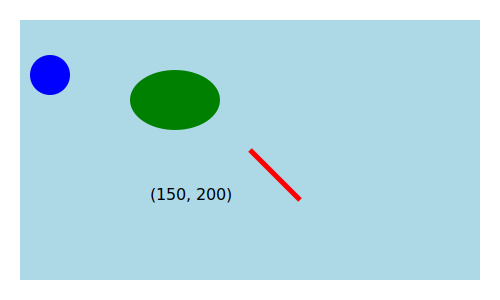
\includegraphics[width=1\linewidth]{images/shapes} \end{center}

Of note:

\begin{itemize}
\item
  An HTML document is composed of lines or sections set off with tags. In particular \texttt{\textless{}style\textgreater{}\ ...\ \textless{}/style\textgreater{}}, \texttt{\textless{}svg\textgreater{}\ ...\ \textless{}/svg\textgreater{}}, and \texttt{\textless{}script\textgreater{}\ ...\ \textless{}/script\textgreater{}} indicate the inclusion of CSS, SVG, and JavaScript/D3 respectively.
\item
  For D3 to work, you must link to a D3 library. To link to the online version, copy and paste the \texttt{\textless{}script\textgreater{}} line from \url{https://d3js.org}. Alternatively, you can also download a copy from the same site and reference your local copy with:

\begin{Shaded}
\begin{Highlighting}[]
\OperatorTok{<}\NormalTok{script src}\OperatorTok{=}\StringTok{"d3.js"}\OperatorTok{>}\NormalTok{</script}\OperatorTok{>}
\end{Highlighting}
\end{Shaded}
\item
  There are two main sections. The \texttt{\textless{}head\textgreater{}} section contains the \emph{title}, \emph{link to D3 library}, and \emph{internal CSS}. The \texttt{\textless{}body\textgreater{}} section contains HTML elements (\texttt{\textless{}h1\textgreater{}}, \texttt{\textless{}p\textgreater{}}, etc.), SVGs (between \texttt{\textless{}svg\textgreater{}}/\texttt{\textless{}/svg\textgreater{}}tags) and JavaScript/D3 scripts (between \texttt{\textless{}script\textgreater{}}/\texttt{\textless{}script\textgreater{}}tags).
\end{itemize}

\begin{quote}
 \emph{Do not assume that if it works that it is correct; today's browsers can be very forgiving.}
\end{quote}

\begin{itemize}
\item
  Comment syntax varies with language:

  \begin{itemize}
  \item
    \texttt{\textless{}!-\/-\ single\ or\ multiline\ HTML\ or\ SVG\ comment\ -\/-\textgreater{}}
  \item
    \texttt{/*\ single\ or\ multiline\ CSS\ comment\ */}
  \item
    \texttt{//\ single\ line\ JavaScript\ comment}
  \item
    \texttt{/*\ JavaScript} \texttt{multiline\ comment\ */}
  \end{itemize}
\end{itemize}

\hypertarget{exercise-shapes}{%
\section{Exercise : shapes}\label{exercise-shapes}}

Download a fresh copy of \texttt{shapes.html}. (Reminder: open the following page and then click \emph{File, Save Page As\ldots{}}: \href{https://raw.githubusercontent.com/jtr13/d3book/master/code/shapes.html}{\texttt{shapes.html}}). Open the file in a text editor of your choice on one half of your screen. If you don't want to think about it, just use RStudio since it's already installed and provides syntax highlighting for \texttt{.html}. On the other half of your screen open the same file in Chrome. Developer Tools should not be open; we will not be using the Console. As you make changes to the \texttt{.html} file, save the file and then refresh the browser to see the effects. Keyboard shortcuts to save and refresh are helpful here.

Your screen should look like this:

\begin{center}\includegraphics[width=0.8\linewidth]{images/editor_chrome} \end{center}

\begin{enumerate}
\def\labelenumi{\arabic{enumi}.}
\item
  Add an additional circle to the svg.
\item
  Add styling to the internal style sheet to style circles.
\item
  Add two additional paragraphs use the \texttt{\textless{}p\textgreater{}} tag.
\item
  Add an ID attribute to one of the circles.
\item
  Add a class attribute to two of the \texttt{\textless{}p\textgreater{}} tags.
\item
  Use the internal style sheet to style paragraphs of the class you created in 5.
\item
  Adjust additional elements as desired.
\end{enumerate}

\protect\hyperlink{web-tech-shapes}{}

\hypertarget{d3console}{%
\chapter{D3 in the Console }\label{d3console}}

Read \emph{IDVW2}, Chapter 6: Drawing with Data. Skip pp.~89-96 as we will not be drawing bar charts with the \texttt{div}approach.

\hypertarget{selections}{%
\section{Selections }\label{selections}}

\hypertarget{select-by-tag}{%
\subsection{Select by tag}\label{select-by-tag}}

The ability to select elements on a page is key to being able to manipulate them. \texttt{d3.select()} will select the first match; \texttt{d3.selectAll()} will select all matches.

\begin{Shaded}
\begin{Highlighting}[]
\VariableTok{d3}\NormalTok{.}\AttributeTok{select}\NormalTok{(}\StringTok{"svg"}\NormalTok{).}\AttributeTok{select}\NormalTok{(}\StringTok{"circle"}\NormalTok{)}\OperatorTok{;}
\end{Highlighting}
\end{Shaded}

selects the first circle in the order in which circles appear in the \texttt{\textless{}svg\textgreater{}} grouping. If there were more than one circle we could select them all with:

\begin{Shaded}
\begin{Highlighting}[]
\VariableTok{d3}\NormalTok{.}\AttributeTok{select}\NormalTok{(}\StringTok{"svg"}\NormalTok{).}\AttributeTok{selectAll}\NormalTok{(}\StringTok{"circle"}\NormalTok{)}\OperatorTok{;}
\end{Highlighting}
\end{Shaded}

We can select HTML elements by tag in the same way:

\begin{Shaded}
\begin{Highlighting}[]
\VariableTok{d3}\NormalTok{.}\AttributeTok{select}\NormalTok{(}\StringTok{"body"}\NormalTok{).}\AttributeTok{select}\NormalTok{(}\StringTok{"h1"}\NormalTok{)}\OperatorTok{;}
\VariableTok{d3}\NormalTok{.}\AttributeTok{select}\NormalTok{(}\StringTok{"body"}\NormalTok{).}\AttributeTok{selectAll}\NormalTok{(}\StringTok{"h1"}\NormalTok{)}\OperatorTok{;}
\end{Highlighting}
\end{Shaded}

\hypertarget{select-by-class}{%
\subsection{Select by class}\label{select-by-class}}

Classes are selected by adding a ``.'' before the class name:

\begin{Shaded}
\begin{Highlighting}[]
\VariableTok{d3}\NormalTok{.}\AttributeTok{select}\NormalTok{(}\StringTok{"svg"}\NormalTok{).}\AttributeTok{selectAll}\NormalTok{(}\StringTok{"circle.apple"}\NormalTok{)}
\end{Highlighting}
\end{Shaded}

This provides one method of selecting a certain collection of elements of the same type.

\hypertarget{select-by-id}{%
\subsection{Select by ID}\label{select-by-id}}

IDs differ from classes in that they are unique identifies. IDs are selected by adding a ``\#'' before the ID:

\begin{Shaded}
\begin{Highlighting}[]
\VariableTok{d3}\NormalTok{.}\AttributeTok{select}\NormalTok{(}\StringTok{"svg"}\NormalTok{).}\AttributeTok{select}\NormalTok{(}\StringTok{"circle#henry"}\NormalTok{)}\OperatorTok{;}
\end{Highlighting}
\end{Shaded}

\hypertarget{store-selections}{%
\subsection{Store selections}\label{store-selections}}

It is often helpful to store selections for later use. Here we store the svg selection in \texttt{mysvg}:

\begin{Shaded}
\begin{Highlighting}[]
\KeywordTok{var}\NormalTok{ mysvg }\OperatorTok{=} \VariableTok{d3}\NormalTok{.}\AttributeTok{select}\NormalTok{(}\StringTok{"svg"}\NormalTok{)}\OperatorTok{;}
\end{Highlighting}
\end{Shaded}

\begin{quote}
 \emph{The JavaScript community is moving toward using \texttt{let} and \texttt{const} instead of \texttt{var}; we, however, will stick with \texttt{var} to be consistent with }IDVW2\emph{. Of course you're welcome to use \texttt{const} and \texttt{let} instead, and if so, may find these articles helpful: \href{https://madhatted.com/2016/1/25/let-it-be}{Let It Be - How to declare JavaScript variables} and \href{https://mathiasbynens.be/notes/es6-const}{ES2015 const is not about immutability}.}
\end{quote}

Store circle selection in a variable:

\begin{Shaded}
\begin{Highlighting}[]
\KeywordTok{var}\NormalTok{ svg }\OperatorTok{=} \VariableTok{d3}\NormalTok{.}\AttributeTok{select}\NormalTok{(}\StringTok{"svg"}\NormalTok{)}\OperatorTok{;}

\KeywordTok{var}\NormalTok{ circ }\OperatorTok{=} \VariableTok{svg}\NormalTok{.}\AttributeTok{selectAll}\NormalTok{(}\StringTok{"circle"}\NormalTok{)}\OperatorTok{;}
\end{Highlighting}
\end{Shaded}

\hypertarget{modify-existing-elements}{%
\section{Modify existing elements }\label{modify-existing-elements}}

Try out the code in this section with a downloaded copy of \href{https://raw.githubusercontent.com/jtr13/d3book/master/code/five_green_circles.html}{five\_green\_circles.html} opened in Chrome and the Console visible.

\hypertarget{modify-attributes}{%
\subsection{Modify attributes}\label{modify-attributes}}

\href{https://github.com/d3/d3-selection/blob/v1.4.0/README.md\#selection_attr}{link to get or set attribute API}

\begin{Shaded}
\begin{Highlighting}[]
\VariableTok{d3}\NormalTok{.}\AttributeTok{select}\NormalTok{(}\StringTok{"circle"}\NormalTok{).}\AttributeTok{attr}\NormalTok{(}\StringTok{"r"}\NormalTok{)}\OperatorTok{;}           \CommentTok{// see radius}

\VariableTok{d3}\NormalTok{.}\AttributeTok{select}\NormalTok{(}\StringTok{"circle"}\NormalTok{).}\AttributeTok{attr}\NormalTok{(}\StringTok{"r"}\OperatorTok{,} \StringTok{"10"}\NormalTok{)}\OperatorTok{;}     \CommentTok{// set radius to 10}
\end{Highlighting}
\end{Shaded}

\hypertarget{modify-styles}{%
\subsection{Modify styles}\label{modify-styles}}

\href{https://github.com/d3/d3-selection/blob/v1.4.0/README.md\#selection_style}{link to get or set style API}

\begin{Shaded}
\begin{Highlighting}[]
\VariableTok{d3}\NormalTok{.}\AttributeTok{select}\NormalTok{(}\StringTok{"h1"}\NormalTok{).}\AttributeTok{style}\NormalTok{(}\StringTok{"color"}\NormalTok{)}\OperatorTok{;}

\VariableTok{d3}\NormalTok{.}\AttributeTok{select}\NormalTok{(}\StringTok{"h1"}\NormalTok{).}\AttributeTok{style}\NormalTok{(}\StringTok{"color"}\OperatorTok{,} \StringTok{"blue"}\NormalTok{)}\OperatorTok{;}
\end{Highlighting}
\end{Shaded}

\begin{quote}
 \emph{It is often difficult to remember whether to use \texttt{.attr()} or \texttt{.style()} In general, properties such as position on the SVG, class, and ID are }attributes\emph{, while decorative properties such as color, font, font size, etc. are }styles\emph{. However, in some cases, you can use either. For example, the following both make the circle blue:}
\end{quote}

\begin{Shaded}
\begin{Highlighting}[]
\VariableTok{d3}\NormalTok{.}\AttributeTok{select}\NormalTok{(}\StringTok{"circle"}\NormalTok{).}\AttributeTok{attr}\NormalTok{(}\StringTok{"fill"}\OperatorTok{,} \StringTok{"blue"}\NormalTok{)}\OperatorTok{;}

\VariableTok{d3}\NormalTok{.}\AttributeTok{select}\NormalTok{(}\StringTok{"circle"}\NormalTok{).}\AttributeTok{style}\NormalTok{(}\StringTok{"fill"}\OperatorTok{,} \StringTok{"blue"}\NormalTok{)}\OperatorTok{;}
\end{Highlighting}
\end{Shaded}

\emph{The first will add a \texttt{fill="blue"} attribute to the \texttt{\textless{}circle\textgreater{}} tag, while the latter will add \texttt{style="fill:\ blue;"}. All is well and good until you find yourself with both in the same tag, in which case the \texttt{style} property will take precedence. The bottom line: don't mix the two options because it can cause problems.}

\begin{quote}
 \emph{To further complicate matters, \texttt{.style()} is just shorthand for \texttt{.attr("style",\ "...")} so the following are in fact equivalent:}
\end{quote}

\begin{Shaded}
\begin{Highlighting}[]
\VariableTok{d3}\NormalTok{.}\AttributeTok{select}\NormalTok{(}\StringTok{"circle"}\NormalTok{).}\AttributeTok{style}\NormalTok{(}\StringTok{"fill"}\OperatorTok{,} \StringTok{"blue"}\NormalTok{)}\OperatorTok{;}

\VariableTok{d3}\NormalTok{.}\AttributeTok{select}\NormalTok{(}\StringTok{"circle"}\NormalTok{).}\AttributeTok{attr}\NormalTok{(}\StringTok{"style"}\OperatorTok{,} \StringTok{"fill: blue;"}\NormalTok{)}\OperatorTok{;}
\end{Highlighting}
\end{Shaded}

\emph{In other words, style is an attribute!}

\hypertarget{modify-text}{%
\subsection{Modify text}\label{modify-text}}

This section is interactive. Hover over code as directed to observe effects.

\hypertarget{html-text}{%
\subsubsection*{HTML text}\label{html-text}}
\addcontentsline{toc}{subsubsection}{HTML text}

\begin{Shaded}
\begin{Highlighting}[]
\KeywordTok{<p}\OtherTok{ id=}\StringTok{"typo"}\OtherTok{ class=}\StringTok{"fancy"}\KeywordTok{>}\NormalTok{Manhatten}\KeywordTok{</p>}
\end{Highlighting}
\end{Shaded}

Manhatten

Hover to execute this code (and fix the typo):

\hypertarget{fixtypo}{}
\begin{Shaded}
\begin{Highlighting}[]
\VariableTok{d3}\NormalTok{.}\AttributeTok{select}\NormalTok{(}\StringTok{"#typo"}\NormalTok{).}\AttributeTok{text}\NormalTok{(}\StringTok{"Manhattan"}\NormalTok{)}\OperatorTok{;}
\end{Highlighting}
\end{Shaded}

\hypertarget{svg-text}{%
\subsubsection*{SVG text}\label{svg-text}}
\addcontentsline{toc}{subsubsection}{SVG text}

\begin{Shaded}
\begin{Highlighting}[]
\KeywordTok{<svg}\OtherTok{ width=}\StringTok{"500"}\OtherTok{ height=}\StringTok{"100"}\KeywordTok{>}
  \KeywordTok{<rect}\OtherTok{ width=}\StringTok{"500"}\OtherTok{ height=}\StringTok{"100"}\OtherTok{ fill=}\StringTok{"#326EA4"}\KeywordTok{></rect>}
  \KeywordTok{<text}\OtherTok{ id=}\StringTok{"svgtypo"}\OtherTok{ x=}\StringTok{"50"}\OtherTok{ y=}\StringTok{"70"}\OtherTok{ fill=}\StringTok{"white"}\OtherTok{ font-weight=}\StringTok{"bold"}\OtherTok{ font-size=}\StringTok{"40px"}\KeywordTok{>}
\NormalTok{     Web scrapping is fun.}\KeywordTok{</text>}
\KeywordTok{</svg>}  
\end{Highlighting}
\end{Shaded}

Hover on this SVG to execute the code below it (and fix the typo):

Web scrapping is fun.

\hypertarget{fixsvgtypo}{}
\begin{Shaded}
\begin{Highlighting}[]
\VariableTok{d3}\NormalTok{.}\AttributeTok{select}\NormalTok{(}\StringTok{"#svgtypo"}\NormalTok{).}\AttributeTok{text}\NormalTok{(}\StringTok{"Web scraping is fun."}\NormalTok{)}\OperatorTok{;}
\end{Highlighting}
\end{Shaded}

\begin{quote}
 \emph{The SVG \texttt{\textless{}text\textgreater{}} tag can be tricky. It differs from HTML text tags (\texttt{\textless{}p\textgreater{},\ \textless{}h1\textgreater{},\ \textless{}h2\textgreater{},} etc.) in that it has \texttt{x} and \texttt{y} attributes that allow you to position text on an SVG canvas. Unlike HTML, the fill attribute controls the color of the text. Compare:}
\end{quote}

\begin{Shaded}
\begin{Highlighting}[]
\VariableTok{d3}\NormalTok{.}\AttributeTok{select}\NormalTok{(}\StringTok{"p"}\NormalTok{).}\AttributeTok{style}\NormalTok{(}\StringTok{"color"}\OperatorTok{,} \StringTok{"red"}\NormalTok{)}\OperatorTok{;}   \CommentTok{// HTML}

\VariableTok{d3}\NormalTok{.}\AttributeTok{select}\NormalTok{(}\StringTok{"text"}\NormalTok{).}\AttributeTok{attr}\NormalTok{(}\StringTok{"fill"}\OperatorTok{,} \StringTok{"red"}\NormalTok{)}\OperatorTok{;}  \CommentTok{// SVG}
\end{Highlighting}
\end{Shaded}

\hypertarget{move-svg-text}{%
\subsection{Move SVG text}\label{move-svg-text}}

\begin{Shaded}
\begin{Highlighting}[]
\KeywordTok{<svg}\OtherTok{ width=}\StringTok{"600"}\OtherTok{ height=}\StringTok{"100"}\KeywordTok{>}
  \KeywordTok{<rect}\OtherTok{ width=}\StringTok{"600"}\OtherTok{ height=}\StringTok{"100"}\OtherTok{ fill=}\StringTok{"#326EA4"}\KeywordTok{></rect>}
  \KeywordTok{<text}\OtherTok{ id=}\StringTok{"moveleft"}\OtherTok{ x=}\StringTok{"200"}\OtherTok{ y=}\StringTok{"70"}\OtherTok{ fill=}\StringTok{"white"}\OtherTok{ font-weight=}\StringTok{"bold"}\OtherTok{ font-size=}\StringTok{"40px"}\KeywordTok{>}
\NormalTok{      I want to move left.}\KeywordTok{</text>}
\KeywordTok{</svg>}  
\end{Highlighting}
\end{Shaded}

Hover on this SVG to execute the code below it:

I want to move left.

\hypertarget{move}{}
\begin{Shaded}
\begin{Highlighting}[]
\VariableTok{d3}\NormalTok{.}\AttributeTok{select}\NormalTok{(}\StringTok{"#moveleft"}\NormalTok{).}\AttributeTok{attr}\NormalTok{(}\StringTok{"x"}\OperatorTok{,} \StringTok{"20"}\NormalTok{).}\AttributeTok{text}\NormalTok{(}\StringTok{"Thanks, now I'm happy!"}\NormalTok{)}\OperatorTok{;}
\end{Highlighting}
\end{Shaded}

\hypertarget{add-elements}{%
\section{Add elements }\label{add-elements}}

\hypertarget{html-1}{%
\subsection{HTML}\label{html-1}}

Continue trying out code with \texttt{five\_green\_circles.html} open in Chrome.

The following adds a \texttt{\textless{}p\textgreater{}} tag but doesn't change how the page looks, since there's no text associated with it.

\begin{Shaded}
\begin{Highlighting}[]
\VariableTok{d3}\NormalTok{.}\AttributeTok{select}\NormalTok{(}\StringTok{"body"}\NormalTok{).}\AttributeTok{append}\NormalTok{(}\StringTok{"p"}\NormalTok{)}\OperatorTok{;}
\end{Highlighting}
\end{Shaded}

To add text, use \texttt{.text()}:

\begin{Shaded}
\begin{Highlighting}[]
\VariableTok{d3}\NormalTok{.}\AttributeTok{select}\NormalTok{(}\StringTok{"body"}\NormalTok{).}\AttributeTok{append}\NormalTok{(}\StringTok{"p"}\NormalTok{).}\AttributeTok{text}\NormalTok{(}\StringTok{"This is a complete sentence."}\NormalTok{)}\OperatorTok{;}
\end{Highlighting}
\end{Shaded}

\begin{quote}
 \emph{To debug adding an element, go to the Elements tab to see what was added and where. If an element is in the wrong place in the HTML tree, it will not be visible.}
\end{quote}

\hypertarget{svg-1}{%
\subsection{SVG}\label{svg-1}}

Likewise, here we add a \texttt{\textless{}circle\textgreater{}} to the \texttt{\textless{}svg\textgreater{}}, but we can't see it since it has no attributes.

\begin{Shaded}
\begin{Highlighting}[]
\VariableTok{d3}\NormalTok{.}\AttributeTok{select}\NormalTok{(}\StringTok{"svg"}\NormalTok{).}\AttributeTok{append}\NormalTok{(}\StringTok{"circle"}\NormalTok{)}\OperatorTok{;}
\end{Highlighting}
\end{Shaded}

Adding attributes will create visible circles:

\begin{Shaded}
\begin{Highlighting}[]
\VariableTok{d3}\NormalTok{.}\AttributeTok{select}\NormalTok{(}\StringTok{"svg"}\NormalTok{).}\AttributeTok{append}\NormalTok{(}\StringTok{"rect"}\NormalTok{).}\AttributeTok{attr}\NormalTok{(}\StringTok{"x"}\OperatorTok{,} \StringTok{"0"}\NormalTok{).}\AttributeTok{attr}\NormalTok{(}\StringTok{"y"}\OperatorTok{,} \StringTok{"0"}\NormalTok{)}
\NormalTok{    .}\AttributeTok{attr}\NormalTok{(}\StringTok{"width"}\OperatorTok{,} \StringTok{"500"}\NormalTok{).}\AttributeTok{attr}\NormalTok{(}\StringTok{"height"}\OperatorTok{,} \StringTok{"400"}\NormalTok{).}\AttributeTok{attr}\NormalTok{(}\StringTok{"fill"}\OperatorTok{,} \StringTok{"lightblue"}\NormalTok{)}\OperatorTok{;}
    
\VariableTok{d3}\NormalTok{.}\AttributeTok{select}\NormalTok{(}\StringTok{"svg"}\NormalTok{).}\AttributeTok{append}\NormalTok{(}\StringTok{"circle"}\NormalTok{).}\AttributeTok{attr}\NormalTok{(}\StringTok{"cx"}\OperatorTok{,} \StringTok{"200"}\NormalTok{)}
\NormalTok{    .}\AttributeTok{attr}\NormalTok{(}\StringTok{"cy"}\OperatorTok{,} \StringTok{"100"}\NormalTok{).}\AttributeTok{attr}\NormalTok{(}\StringTok{"r"}\OperatorTok{,} \StringTok{"25"}\NormalTok{).}\AttributeTok{attr}\NormalTok{(}\StringTok{"fill"}\OperatorTok{,} \StringTok{"orange"}\NormalTok{)}\OperatorTok{;}
    
\VariableTok{d3}\NormalTok{.}\AttributeTok{select}\NormalTok{(}\StringTok{"svg"}\NormalTok{).}\AttributeTok{append}\NormalTok{(}\StringTok{"circle"}\NormalTok{).}\AttributeTok{attr}\NormalTok{(}\StringTok{"cx"}\OperatorTok{,} \StringTok{"300"}\NormalTok{)}
\NormalTok{    .}\AttributeTok{attr}\NormalTok{(}\StringTok{"cy"}\OperatorTok{,} \StringTok{"150"}\NormalTok{).}\AttributeTok{attr}\NormalTok{(}\StringTok{"r"}\OperatorTok{,} \StringTok{"25"}\NormalTok{).}\AttributeTok{attr}\NormalTok{(}\StringTok{"fill"}\OperatorTok{,} \StringTok{"red"}\NormalTok{)}\OperatorTok{;}  
\end{Highlighting}
\end{Shaded}

We can use a saved selection to assist in creating a new element:

(\emph{IDVW2}, pp.~97-98)

\begin{Shaded}
\begin{Highlighting}[]
\NormalTok{mysvg }\OperatorTok{=} \VariableTok{d3}\NormalTok{.}\AttributeTok{select}\NormalTok{(}\StringTok{"svg"}\NormalTok{)}\OperatorTok{;}

\VariableTok{mysvg}\NormalTok{.}\AttributeTok{append}\NormalTok{(}\StringTok{"circle"}\NormalTok{).}\AttributeTok{attr}\NormalTok{(}\StringTok{"cx"}\OperatorTok{,} \StringTok{"250"}\NormalTok{).}\AttributeTok{attr}\NormalTok{(}\StringTok{"cy"}\OperatorTok{,} \StringTok{"250"}\NormalTok{).}\AttributeTok{attr}\NormalTok{(}\StringTok{"r"}\OperatorTok{,} \StringTok{"50"}\NormalTok{)}
\NormalTok{  .}\AttributeTok{attr}\NormalTok{(}\StringTok{"fill"}\OperatorTok{,} \StringTok{"red"}\NormalTok{)}\OperatorTok{;}
\end{Highlighting}
\end{Shaded}

\hypertarget{remove-elements}{%
\section{Remove elements }\label{remove-elements}}

These methods will remove matching elements in order, starting with the first find in the document.

\hypertarget{html-2}{%
\subsection{HTML}\label{html-2}}

\begin{Shaded}
\begin{Highlighting}[]
\VariableTok{d3}\NormalTok{.}\AttributeTok{select}\NormalTok{(}\StringTok{"p"}\NormalTok{).}\AttributeTok{remove}\NormalTok{()}\OperatorTok{;}
\end{Highlighting}
\end{Shaded}

\hypertarget{svg-2}{%
\subsection{SVG}\label{svg-2}}

\begin{Shaded}
\begin{Highlighting}[]
\VariableTok{d3}\NormalTok{.}\AttributeTok{select}\NormalTok{(}\StringTok{"svg"}\NormalTok{).}\AttributeTok{select}\NormalTok{(}\StringTok{"circle"}\NormalTok{).}\AttributeTok{remove}\NormalTok{()}\OperatorTok{;}

\VariableTok{d3}\NormalTok{.}\AttributeTok{select}\NormalTok{(}\StringTok{"svg"}\NormalTok{).}\AttributeTok{selectAll}\NormalTok{(}\StringTok{"circle"}\NormalTok{).}\AttributeTok{remove}\NormalTok{()}\OperatorTok{;}
\end{Highlighting}
\end{Shaded}

\hypertarget{exercise-green-circles}{%
\section{Exercise : green circles}\label{exercise-green-circles}}

Download and open a fresh copy of \href{https://raw.githubusercontent.com/jtr13/d3book/master/code/five_green_circles.html}{five\_green\_circles.html} in Chrome. Open Developer Tools open and do the following in the Console with D3:

\begin{enumerate}
\def\labelenumi{\arabic{enumi}.}
\item
  Select the circle with ID ``henry'' and make it blue.
\item
  Select all circles of ``apple'' class make them red.
\item
  Select the first circle and add an orange border (``stroke''), and stroke width (``stroke-width'') of 5.
\item
  Select all circles of ``apple'' class and move them to the middle of the svg.
\end{enumerate}

\protect\hyperlink{d3-in-the-console-green-circles}{}

\hypertarget{exercise-blue-circles}{%
\section{\texorpdfstring{Exercise : blue circles}{Exercise  : blue circles}}\label{exercise-blue-circles}}

Download and open a fresh copy of \href{https://raw.githubusercontent.com/jtr13/d3book/master/code/six_blue_circles.html}{six\_blue\_circles.html} in Chrome. Open Developer Tools and execute Steps 1-4 one at a time in the Console. After Step 4, refresh the page to go back to Step 1 if so desired. (You do not need to create a loop as in the visual.)

\begin{quote}
 \emph{This exercise is provided as a challenge. It's fine to skip this exercise and move on to the next section.}
\end{quote}

\begin{enumerate}
\def\labelenumi{\arabic{enumi}.}
\item
  Move all the circles to the right.
\item
  Move them back to the left \emph{and} change their color.
\item
  In a text editor, add an id to the third circle in \texttt{six\_blue\_circles.html}, save the file, and then in the Console, move only that circle to the right.
\item
  Move all the circles to the middle of the screen, \emph{then} move them all to the same location.
\end{enumerate}

\protect\hyperlink{d3-in-the-console-blue-circles}{}

\hypertarget{bind-data-finally}{%
\section{\texorpdfstring{Bind data\ldots{} \emph{finally!} }{Bind data\ldots{} finally! }}\label{bind-data-finally}}

(\emph{IDVW2}, pp.~98-108)

To follow along with the code in this section, download and open \href{https://raw.githubusercontent.com/jtr13/d3book/master/code/six_blue_circles.html}{six\_blue\_circles.html}.

Bind data:

\begin{Shaded}
\begin{Highlighting}[]
\VariableTok{d3}\NormalTok{.}\AttributeTok{select}\NormalTok{(}\StringTok{"svg"}\NormalTok{).}\AttributeTok{selectAll}\NormalTok{(}\StringTok{"circle"}\NormalTok{).}\AttributeTok{data}\NormalTok{([}\DecValTok{90}\OperatorTok{,} \DecValTok{230}\OperatorTok{,} \DecValTok{140}\OperatorTok{,} \DecValTok{75}\OperatorTok{,} \DecValTok{180}\OperatorTok{,} \DecValTok{25}\NormalTok{])}\OperatorTok{;}
\end{Highlighting}
\end{Shaded}

Check data binding:

\begin{Shaded}
\begin{Highlighting}[]
\VariableTok{d3}\NormalTok{.}\AttributeTok{select}\NormalTok{(}\StringTok{"svg"}\NormalTok{).}\AttributeTok{selectAll}\NormalTok{(}\StringTok{"circle"}\NormalTok{).}\AttributeTok{data}\NormalTok{()}\OperatorTok{;}
\end{Highlighting}
\end{Shaded}

Set x-coordinate of each circle to data value using arrow function:

\begin{Shaded}
\begin{Highlighting}[]
\VariableTok{d3}\NormalTok{.}\AttributeTok{select}\NormalTok{(}\StringTok{"svg"}\NormalTok{).}\AttributeTok{selectAll}\NormalTok{(}\StringTok{"circle"}\NormalTok{).}\AttributeTok{attr}\NormalTok{(}\StringTok{"cx"}\OperatorTok{,}\NormalTok{ d }\OperatorTok{=>}\NormalTok{ d)}\OperatorTok{;}
\end{Highlighting}
\end{Shaded}

Set x-coordinate of each circle to data value with a JavaScript function:

\begin{Shaded}
\begin{Highlighting}[]
\VariableTok{d3}\NormalTok{.}\AttributeTok{select}\NormalTok{(}\StringTok{"svg"}\NormalTok{).}\AttributeTok{selectAll}\NormalTok{(}\StringTok{"circle"}\NormalTok{).}\AttributeTok{attr}\NormalTok{(}\StringTok{"cx"}\OperatorTok{,} \KeywordTok{function}\NormalTok{(d) }\OperatorTok{\{}\ControlFlowTok{return}\NormalTok{ d}\OperatorTok{;\}}\NormalTok{)}\OperatorTok{;}
\end{Highlighting}
\end{Shaded}

We'll bind a new set of data to the circles, this time storying the dataset in a variable:

\begin{Shaded}
\begin{Highlighting}[]
\KeywordTok{var}\NormalTok{ dataset }\OperatorTok{=}\NormalTok{ [}\DecValTok{50}\OperatorTok{,} \DecValTok{80}\OperatorTok{,} \DecValTok{110}\OperatorTok{,} \DecValTok{140}\OperatorTok{,} \DecValTok{170}\OperatorTok{,} \DecValTok{200}\NormalTok{]}\OperatorTok{;}
\end{Highlighting}
\end{Shaded}

We'll also store a selection of all circles before binding the data:

\begin{Shaded}
\begin{Highlighting}[]
\KeywordTok{var}\NormalTok{ circ }\OperatorTok{=} \VariableTok{d3}\NormalTok{.}\AttributeTok{select}\NormalTok{(}\StringTok{"svg"}\NormalTok{).}\AttributeTok{selectAll}\NormalTok{(}\StringTok{"circle"}\NormalTok{)}\OperatorTok{;}
\end{Highlighting}
\end{Shaded}

And now, the data bind:

\begin{Shaded}
\begin{Highlighting}[]
\VariableTok{circ}\NormalTok{.}\AttributeTok{data}\NormalTok{(dataset)}\OperatorTok{;}
\end{Highlighting}
\end{Shaded}

Nothing appears to have happened; the circles remain the same and there is no evidence of any changes looking at the circles in the DOM (see Elements tab).

We can check that the data are indeed bound with:

\begin{Shaded}
\begin{Highlighting}[]
\VariableTok{circ}\NormalTok{.}\AttributeTok{data}\NormalTok{()}\OperatorTok{;}  \CommentTok{// now we see data}
\end{Highlighting}
\end{Shaded}

Modify elements w/ stored selections, bound data:

\begin{Shaded}
\begin{Highlighting}[]
\VariableTok{circ}\NormalTok{.}\AttributeTok{attr}\NormalTok{(}\StringTok{"cx"}\OperatorTok{,} \KeywordTok{function}\NormalTok{(d) }\OperatorTok{\{}\ControlFlowTok{return}\NormalTok{ d}\OperatorTok{;\}}\NormalTok{)}\OperatorTok{;}

\VariableTok{circ}\NormalTok{.}\AttributeTok{attr}\NormalTok{(}\StringTok{"cx"}\OperatorTok{,} \KeywordTok{function}\NormalTok{(d) }\OperatorTok{\{}\ControlFlowTok{return}\NormalTok{ d/}\DecValTok{2}\OperatorTok{;\}}\NormalTok{)}\OperatorTok{;}

\VariableTok{circ}\NormalTok{.}\AttributeTok{attr}\NormalTok{(}\StringTok{"cx"}\OperatorTok{,} \KeywordTok{function}\NormalTok{(d) }\OperatorTok{\{}\ControlFlowTok{return}\NormalTok{ d/}\DecValTok{4}\OperatorTok{;\}}\NormalTok{).}\AttributeTok{attr}\NormalTok{(}\StringTok{"r"}\OperatorTok{,} \StringTok{"10"}\NormalTok{)}\OperatorTok{;}
\end{Highlighting}
\end{Shaded}

Same as above, using arrow functions:

\begin{Shaded}
\begin{Highlighting}[]
\VariableTok{circ}\NormalTok{.}\AttributeTok{attr}\NormalTok{(}\StringTok{"cx"}\OperatorTok{,}\NormalTok{ d }\OperatorTok{=>}\NormalTok{ d)}\OperatorTok{;}

\VariableTok{circ}\NormalTok{.}\AttributeTok{attr}\NormalTok{(}\StringTok{"cx"}\OperatorTok{,}\NormalTok{ d }\OperatorTok{=>}\NormalTok{ d/}\DecValTok{2}\NormalTok{)}\OperatorTok{;}

\VariableTok{circ}\NormalTok{.}\AttributeTok{attr}\NormalTok{(}\StringTok{"r"}\OperatorTok{,}\NormalTok{ d }\OperatorTok{=>}\NormalTok{ d/}\DecValTok{4}\NormalTok{).}\AttributeTok{attr}\NormalTok{(}\StringTok{"r"}\OperatorTok{,} \StringTok{"10"}\NormalTok{)}\OperatorTok{;}
\end{Highlighting}
\end{Shaded}

Note that if we bind a new set of data to the DOM elements, the original set will be overwritten:

\begin{Shaded}
\begin{Highlighting}[]
\KeywordTok{var}\NormalTok{ newdata }\OperatorTok{=}\NormalTok{ [}\DecValTok{145}\OperatorTok{,} \DecValTok{29}\OperatorTok{,} \DecValTok{53}\OperatorTok{,} \DecValTok{196}\OperatorTok{,} \DecValTok{200}\OperatorTok{,} \DecValTok{12}\NormalTok{]}\OperatorTok{;}

\VariableTok{circ}\NormalTok{.}\AttributeTok{data}\NormalTok{(newdata)}\OperatorTok{;}

\VariableTok{circ}\NormalTok{.}\AttributeTok{transition}\NormalTok{()}
\NormalTok{    .}\AttributeTok{duration}\NormalTok{(}\DecValTok{2000}\NormalTok{)}
\NormalTok{    .}\AttributeTok{attr}\NormalTok{(}\StringTok{"cx"}\OperatorTok{,}\NormalTok{ d }\OperatorTok{=>} \DecValTok{2}\OperatorTok{*}\NormalTok{d)}\OperatorTok{;}
\end{Highlighting}
\end{Shaded}

\hypertarget{exercise-data-bind}{%
\section{Exercise : data bind}\label{exercise-data-bind}}

Download and open a fresh copy of \href{https://raw.githubusercontent.com/jtr13/d3book/master/code/six_blue_circles.html}{six\_blue\_circles.html} in Chrome and practice binding data to the circles and modifying the circles based on the data as in the examples above.

\hypertarget{update-enter-and-exit}{%
\chapter{Update, Enter, and Exit }\label{update-enter-and-exit}}

\emph{IDVW2}, Chapter 9, pp.~178-184; Chapter 12, pp.~231-249

\hypertarget{lecture-slides}{%
\section{Lecture slides }\label{lecture-slides}}

\href{https://github.com/jtr13/D3/blob/master/UpdateEnterExit.pdf}{D3 Data Bind}

\hypertarget{remove-some-elements}{%
\section{Remove some elements }\label{remove-some-elements}}

\emph{a.k.a. more DOM elements than data values}

We'll start with six circles and remove some.

Download and open a fresh copy of \href{https://raw.githubusercontent.com/jtr13/d3book/master/code/six_blue_circles.html}{six\_blue\_circles.html} in Chrome.

Let's bind four data values to the six circles:

\begin{Shaded}
\begin{Highlighting}[]
\KeywordTok{var}\NormalTok{ svg }\OperatorTok{=} \VariableTok{d3}\NormalTok{.}\AttributeTok{select}\NormalTok{(}\StringTok{"svg"}\NormalTok{)}\OperatorTok{;}

\VariableTok{svg}\NormalTok{.}\AttributeTok{selectAll}\NormalTok{(}\StringTok{"circle"}\NormalTok{)}
\NormalTok{    .}\AttributeTok{data}\NormalTok{([}\DecValTok{123}\OperatorTok{,} \DecValTok{52}\OperatorTok{,} \DecValTok{232}\OperatorTok{,} \DecValTok{90}\NormalTok{])}\OperatorTok{;}
\end{Highlighting}
\end{Shaded}

Click the black triangle to view the \texttt{\_enter}, \texttt{\_exit}, and \texttt{\_groups} fields.

We can store the selection in a variable:

\begin{Shaded}
\begin{Highlighting}[]
\KeywordTok{var}\NormalTok{ circ }\OperatorTok{=} \VariableTok{svg}\NormalTok{.}\AttributeTok{selectAll}\NormalTok{(}\StringTok{"circle"}\NormalTok{)}
\NormalTok{    .}\AttributeTok{data}\NormalTok{([}\DecValTok{123}\OperatorTok{,} \DecValTok{52}\OperatorTok{,} \DecValTok{232}\OperatorTok{,} \DecValTok{90}\NormalTok{])}\OperatorTok{;}
\end{Highlighting}
\end{Shaded}

Let's look at the exit selection:

\begin{Shaded}
\begin{Highlighting}[]
\VariableTok{circ}\NormalTok{.}\AttributeTok{exit}\NormalTok{()}\OperatorTok{;}
\end{Highlighting}
\end{Shaded}

Try this:

\begin{Shaded}
\begin{Highlighting}[]
\VariableTok{circ}\NormalTok{.}\AttributeTok{attr}\NormalTok{(}\StringTok{"fill"}\OperatorTok{,} \StringTok{"red"}\NormalTok{)}\OperatorTok{;}
\end{Highlighting}
\end{Shaded}

What happened and why?

Now try this:

\begin{Shaded}
\begin{Highlighting}[]
\VariableTok{circ}\NormalTok{.}\AttributeTok{exit}\NormalTok{().}\AttributeTok{attr}\NormalTok{(}\StringTok{"fill"}\OperatorTok{,} \StringTok{"purple"}\NormalTok{)}\OperatorTok{;}
\end{Highlighting}
\end{Shaded}

What happened and why?

What do you think this will do? Try it.

\begin{Shaded}
\begin{Highlighting}[]
\VariableTok{circ}\NormalTok{.}\AttributeTok{exit}\NormalTok{().}\AttributeTok{transition}\NormalTok{().}\AttributeTok{duration}\NormalTok{(}\DecValTok{2000}\NormalTok{).}\AttributeTok{remove}\NormalTok{()}\OperatorTok{;}
\end{Highlighting}
\end{Shaded}

Create a new variable \texttt{circ2} and compare it to \texttt{circ}:

\begin{Shaded}
\begin{Highlighting}[]
\KeywordTok{var}\NormalTok{ circ2 }\OperatorTok{=} \VariableTok{d3}\NormalTok{.}\AttributeTok{selectAll}\NormalTok{(}\StringTok{"circle"}\NormalTok{)}\OperatorTok{;}

\VariableTok{circ}\NormalTok{.}\AttributeTok{data}\NormalTok{()}\OperatorTok{;}

\VariableTok{circ2}\NormalTok{.}\AttributeTok{data}\NormalTok{()}\OperatorTok{;}

\VariableTok{circ}\NormalTok{.}\AttributeTok{exit}\NormalTok{()}\OperatorTok{;}

\VariableTok{circ2}\NormalTok{.}\AttributeTok{exit}\NormalTok{()}\OperatorTok{;}
\end{Highlighting}
\end{Shaded}

What's going on?

\hypertarget{add-some-elements}{%
\section{Add some elements }\label{add-some-elements}}

\emph{a.k.a. more data values than DOM elements}

We'll start with six circles and add some.

Let's bind new data to the circles:

\begin{Shaded}
\begin{Highlighting}[]
\KeywordTok{var}\NormalTok{ circ }\OperatorTok{=} \VariableTok{svg}\NormalTok{.}\AttributeTok{selectAll}\NormalTok{(}\StringTok{"circle"}\NormalTok{)}
\NormalTok{      .}\AttributeTok{data}\NormalTok{([}\DecValTok{123}\OperatorTok{,} \DecValTok{52}\OperatorTok{,} \DecValTok{232}\OperatorTok{,} \DecValTok{90}\OperatorTok{,} \DecValTok{34}\OperatorTok{,} \DecValTok{12}\OperatorTok{,} \DecValTok{189}\OperatorTok{,} \DecValTok{110}\NormalTok{])}\OperatorTok{;}
\end{Highlighting}
\end{Shaded}

And look at the enter selection:

\begin{Shaded}
\begin{Highlighting}[]
\VariableTok{circ}\NormalTok{.}\AttributeTok{enter}\NormalTok{()}\OperatorTok{;}
\end{Highlighting}
\end{Shaded}

How many placeholders are in the enter selection?

Let's add circles for each of these placeholders:

\begin{Shaded}
\begin{Highlighting}[]
\VariableTok{circ}\NormalTok{.}\AttributeTok{enter}\NormalTok{()}
\NormalTok{    .}\AttributeTok{append}\NormalTok{(}\StringTok{"circle"}\NormalTok{)}
\NormalTok{      .}\AttributeTok{attr}\NormalTok{(}\StringTok{"cx"}\OperatorTok{,} \StringTok{"100"}\NormalTok{)}
\NormalTok{      .}\AttributeTok{attr}\NormalTok{(}\StringTok{"cy"}\OperatorTok{,}\NormalTok{ (d}\OperatorTok{,}\NormalTok{ i) }\OperatorTok{=>}\NormalTok{ i }\OperatorTok{*} \DecValTok{50} \OperatorTok{+} \DecValTok{25}\NormalTok{)}
\NormalTok{      .}\AttributeTok{attr}\NormalTok{(}\StringTok{"r"}\OperatorTok{,} \StringTok{"20"}\NormalTok{)}
\NormalTok{      .}\AttributeTok{attr}\NormalTok{(}\StringTok{"fill"}\OperatorTok{,} \StringTok{"blue"}\NormalTok{)}\OperatorTok{;}
\end{Highlighting}
\end{Shaded}

Try this:

\begin{Shaded}
\begin{Highlighting}[]
\VariableTok{circ}\NormalTok{.}\AttributeTok{transition}\NormalTok{()}
\NormalTok{  .}\AttributeTok{duration}\NormalTok{(}\DecValTok{3000}\NormalTok{)}
\NormalTok{  .}\AttributeTok{attr}\NormalTok{(}\StringTok{"cx"}\OperatorTok{,} \StringTok{"400"}\NormalTok{)}\OperatorTok{;}
\end{Highlighting}
\end{Shaded}

What do you need to do to act on \emph{all} of the circles?

\begin{Shaded}
\begin{Highlighting}[]
\VariableTok{svg}\NormalTok{.}\AttributeTok{selectAll}\NormalTok{(}\StringTok{"circle"}\NormalTok{)}
\NormalTok{  .}\AttributeTok{transition}\NormalTok{()}
\NormalTok{  .}\AttributeTok{duration}\NormalTok{(}\DecValTok{2000}\NormalTok{)}
\NormalTok{  .}\AttributeTok{attr}\NormalTok{(}\StringTok{"cy"}\OperatorTok{,}\NormalTok{ (d}\OperatorTok{,}\NormalTok{ i) }\OperatorTok{=>}\NormalTok{ (i }\OperatorTok{*} \DecValTok{50}\NormalTok{) }\OperatorTok{+} \DecValTok{25}\NormalTok{)}
\NormalTok{  .}\AttributeTok{attr}\NormalTok{(}\StringTok{"cx"}\OperatorTok{,} \StringTok{"200"}\NormalTok{)}\OperatorTok{;}
\end{Highlighting}
\end{Shaded}

\hypertarget{data-enter-append}{%
\section{Data / enter / append }\label{data-enter-append}}

We'll start with nothing--not even an SVG--and add elements with the data / enter / append sequence.

Open Developer Tools and copy and paste the code below in the Console. (Click above to close the table of contents on the left so you'll have more screen space.)

The SVG will be added here:

\hypertarget{dea}{}

\begin{Shaded}
\begin{Highlighting}[]
\KeywordTok{var}\NormalTok{ svg }\OperatorTok{=} \VariableTok{d3}\NormalTok{.}\AttributeTok{select}\NormalTok{(}\StringTok{"div#dea"}\NormalTok{)}
\NormalTok{  .}\AttributeTok{append}\NormalTok{(}\StringTok{"svg"}\NormalTok{)}
\NormalTok{  .}\AttributeTok{attr}\NormalTok{(}\StringTok{"width"}\OperatorTok{,} \StringTok{"400"}\NormalTok{)}
\NormalTok{  .}\AttributeTok{attr}\NormalTok{(}\StringTok{"height"}\OperatorTok{,} \StringTok{"250"}\NormalTok{)}\OperatorTok{;}
\end{Highlighting}
\end{Shaded}

Create an array of values:

\begin{Shaded}
\begin{Highlighting}[]
\KeywordTok{var}\NormalTok{ specialdata }\OperatorTok{=}\NormalTok{ [}\DecValTok{75}\OperatorTok{,} \DecValTok{150}\OperatorTok{,} \DecValTok{200}\NormalTok{]}\OperatorTok{;}
\end{Highlighting}
\end{Shaded}

Add rectangles:

\begin{Shaded}
\begin{Highlighting}[]
  \VariableTok{svg}\NormalTok{.}\AttributeTok{selectAll}\NormalTok{(}\StringTok{"rect"}\NormalTok{)}
\NormalTok{    .}\AttributeTok{data}\NormalTok{(specialdata)}
\NormalTok{    .}\AttributeTok{enter}\NormalTok{()}
\NormalTok{    .}\AttributeTok{append}\NormalTok{(}\StringTok{"rect"}\NormalTok{)}
\NormalTok{      .}\AttributeTok{attr}\NormalTok{(}\StringTok{"x"}\OperatorTok{,}\NormalTok{ d }\OperatorTok{=>}\NormalTok{ d)}
\NormalTok{      .}\AttributeTok{attr}\NormalTok{(}\StringTok{"y"}\OperatorTok{,}\NormalTok{ d }\OperatorTok{=>}\NormalTok{ d)}
\NormalTok{      .}\AttributeTok{attr}\NormalTok{(}\StringTok{"width"}\OperatorTok{,} \StringTok{"50"}\NormalTok{)}
\NormalTok{      .}\AttributeTok{attr}\NormalTok{(}\StringTok{"height"}\OperatorTok{,} \StringTok{"30"}\NormalTok{)}
\NormalTok{      .}\AttributeTok{attr}\NormalTok{(}\StringTok{"fill"}\OperatorTok{,} \StringTok{"pink"}\NormalTok{)}\OperatorTok{;}
\end{Highlighting}
\end{Shaded}

\hypertarget{labels}{%
\subsection{Labels}\label{labels}}

Note that we can also label the rectangles with the data value:

\begin{Shaded}
\begin{Highlighting}[]
  \VariableTok{svg}\NormalTok{.}\AttributeTok{selectAll}\NormalTok{(}\StringTok{"text"}\NormalTok{)}
\NormalTok{      .}\AttributeTok{data}\NormalTok{(specialdata)}
\NormalTok{      .}\AttributeTok{enter}\NormalTok{()}
\NormalTok{      .}\AttributeTok{append}\NormalTok{(}\StringTok{"text"}\NormalTok{)}
\NormalTok{      .}\AttributeTok{attr}\NormalTok{(}\StringTok{"x"}\OperatorTok{,}\NormalTok{ d }\OperatorTok{=>}\NormalTok{ d }\OperatorTok{+} \DecValTok{25}\NormalTok{)}
\NormalTok{      .}\AttributeTok{attr}\NormalTok{(}\StringTok{"y"}\OperatorTok{,}\NormalTok{ d }\OperatorTok{=>}\NormalTok{ d }\OperatorTok{+} \DecValTok{25}\NormalTok{)}
\NormalTok{      .}\AttributeTok{text}\NormalTok{(d }\OperatorTok{=>}\NormalTok{ d)}
\NormalTok{      .}\AttributeTok{attr}\NormalTok{(}\StringTok{"fill"}\OperatorTok{,} \StringTok{"blue"}\NormalTok{)}
\NormalTok{      .}\AttributeTok{attr}\NormalTok{(}\StringTok{"text-anchor"}\OperatorTok{,} \StringTok{"middle"}\NormalTok{)}\OperatorTok{;}
\end{Highlighting}
\end{Shaded}

\hypertarget{exercise-horizontal-bar-chart}{%
\section{Exercise : horizontal bar chart}\label{exercise-horizontal-bar-chart}}

\begin{enumerate}
\def\labelenumi{\arabic{enumi}.}
\tightlist
\item
  Create a new html file (try to recreate the template without looking\ldots{} or save a copy of \href{https://raw.githubusercontent.com/jtr13/d3book/master/code/d3template.html}{this one}) and open it in your text editor.
\end{enumerate}

\begin{quote}
 \emph{If you create a new file in RStudio, choose ``Text File'' and use the \texttt{.html} file extension when you save it. Do not choose ``R HTML''.}
\end{quote}

Add a script that adds an svg element and horizontal bars of the lengths (in pixels) specified in \texttt{bardata}. Create the bars with the data / enter / append sequence.

\begin{Shaded}
\begin{Highlighting}[]
    \KeywordTok{var}\NormalTok{ bardata }\OperatorTok{=}\NormalTok{ [}\DecValTok{300}\OperatorTok{,} \DecValTok{100}\OperatorTok{,} \DecValTok{150}\OperatorTok{,} \DecValTok{225}\OperatorTok{,} \DecValTok{75}\OperatorTok{,} \DecValTok{275}\NormalTok{]}\OperatorTok{;}
\end{Highlighting}
\end{Shaded}

\hypertarget{merge-selections}{%
\section{Merge selections }\label{merge-selections}}

a.k.a. combining update and enter selections with \texttt{.merge()}

Open \href{code/six_blue_circles.html}{six\_blue\_circles.html} in Chrome. (You do not need to download it first.)

Run the following code in the Console:

\begin{Shaded}
\begin{Highlighting}[]
\KeywordTok{var}\NormalTok{ svg }\OperatorTok{=} \VariableTok{d3}\NormalTok{.}\AttributeTok{select}\NormalTok{(}\StringTok{"svg"}\NormalTok{)}\OperatorTok{;}
\KeywordTok{var}\NormalTok{ circ }\OperatorTok{=} \VariableTok{svg}\NormalTok{.}\AttributeTok{selectAll}\NormalTok{(}\StringTok{"circle"}\NormalTok{)}
\NormalTok{  .}\AttributeTok{data}\NormalTok{([}\DecValTok{123}\OperatorTok{,} \DecValTok{52}\OperatorTok{,} \DecValTok{232}\OperatorTok{,} \DecValTok{90}\OperatorTok{,} \DecValTok{34}\OperatorTok{,} \DecValTok{12}\OperatorTok{,} \DecValTok{189}\OperatorTok{,} \DecValTok{110}\NormalTok{])}\OperatorTok{;}
  
\KeywordTok{var}\NormalTok{ allcirc }\OperatorTok{=} \VariableTok{circ}\NormalTok{.}\AttributeTok{enter}\NormalTok{()  }\CommentTok{// 2 placeholders}
\NormalTok{        .}\AttributeTok{append}\NormalTok{(}\StringTok{"circle"}\NormalTok{)  }\CommentTok{// placeholders -> circles}
\NormalTok{          .}\AttributeTok{attr}\NormalTok{(}\StringTok{"cx"}\OperatorTok{,} \StringTok{"100"}\NormalTok{)  }\CommentTok{// acts on enter selection only}
\NormalTok{          .}\AttributeTok{attr}\NormalTok{(}\StringTok{"cy"}\OperatorTok{,}\NormalTok{ (d}\OperatorTok{,}\NormalTok{ i) }\OperatorTok{=>}\NormalTok{ (i }\OperatorTok{-} \DecValTok{5}\NormalTok{) }\OperatorTok{*} \DecValTok{50}\NormalTok{)}
\NormalTok{          .}\AttributeTok{attr}\NormalTok{(}\StringTok{"r"}\OperatorTok{,} \StringTok{"20"}\NormalTok{)}
\NormalTok{          .}\AttributeTok{attr}\NormalTok{(}\StringTok{"fill"}\OperatorTok{,} \StringTok{"red"}\NormalTok{)}\OperatorTok{;}
\end{Highlighting}
\end{Shaded}

Now try to predict what the following code will do. Were you right?

\begin{Shaded}
\begin{Highlighting}[]
\VariableTok{allcirc}\NormalTok{.}\AttributeTok{transition}\NormalTok{() }
\NormalTok{        .}\AttributeTok{duration}\NormalTok{(}\DecValTok{3000}\NormalTok{)}
\NormalTok{        .}\AttributeTok{attr}\NormalTok{(}\StringTok{"cx"}\OperatorTok{,} \StringTok{"400"}\NormalTok{)}
\NormalTok{        .}\AttributeTok{attr}\NormalTok{(}\StringTok{"fill"}\OperatorTok{,} \StringTok{"purple"}\NormalTok{)}\OperatorTok{;}
\end{Highlighting}
\end{Shaded}

Refresh the page and then copy and paste the following into the Console and run.

\begin{Shaded}
\begin{Highlighting}[]
\KeywordTok{var}\NormalTok{ svg }\OperatorTok{=} \VariableTok{d3}\NormalTok{.}\AttributeTok{select}\NormalTok{(}\StringTok{"svg"}\NormalTok{)}\OperatorTok{;}
\KeywordTok{var}\NormalTok{ circ }\OperatorTok{=} \VariableTok{svg}\NormalTok{.}\AttributeTok{selectAll}\NormalTok{(}\StringTok{"circle"}\NormalTok{)}
\NormalTok{  .}\AttributeTok{data}\NormalTok{([}\DecValTok{123}\OperatorTok{,} \DecValTok{52}\OperatorTok{,} \DecValTok{232}\OperatorTok{,} \DecValTok{90}\OperatorTok{,} \DecValTok{34}\OperatorTok{,} \DecValTok{12}\OperatorTok{,} \DecValTok{189}\OperatorTok{,} \DecValTok{110}\NormalTok{])}\OperatorTok{;} \CommentTok{// update selection}
  
\KeywordTok{var}\NormalTok{ allcirc }\OperatorTok{=} \VariableTok{circ}\NormalTok{.}\AttributeTok{enter}\NormalTok{()  }\CommentTok{// 2 placeholders}
\NormalTok{        .}\AttributeTok{append}\NormalTok{(}\StringTok{"circle"}\NormalTok{)  }\CommentTok{// placeholders -> circles}
\NormalTok{          .}\AttributeTok{attr}\NormalTok{(}\StringTok{"cx"}\OperatorTok{,} \StringTok{"100"}\NormalTok{)  }\CommentTok{// acts on enter selection only}
\NormalTok{          .}\AttributeTok{attr}\NormalTok{(}\StringTok{"cy"}\OperatorTok{,}\NormalTok{ (d}\OperatorTok{,}\NormalTok{ i) }\OperatorTok{=>}\NormalTok{ (i }\OperatorTok{-} \DecValTok{5}\NormalTok{) }\OperatorTok{*} \DecValTok{50}\NormalTok{)}
\NormalTok{          .}\AttributeTok{attr}\NormalTok{(}\StringTok{"r"}\OperatorTok{,} \StringTok{"20"}\NormalTok{)}
\NormalTok{          .}\AttributeTok{attr}\NormalTok{(}\StringTok{"fill"}\OperatorTok{,} \StringTok{"red"}\NormalTok{)}
\NormalTok{          .}\AttributeTok{merge}\NormalTok{(circ)}\OperatorTok{;}  \CommentTok{// combines enter and update selections}
\end{Highlighting}
\end{Shaded}

And now, the following code (same as before). What changed? Why?

\begin{Shaded}
\begin{Highlighting}[]
\VariableTok{allcirc}\NormalTok{.}\AttributeTok{transition}\NormalTok{() }
\NormalTok{        .}\AttributeTok{duration}\NormalTok{(}\DecValTok{3000}\NormalTok{)}
\NormalTok{        .}\AttributeTok{attr}\NormalTok{(}\StringTok{"cx"}\OperatorTok{,} \StringTok{"400"}\NormalTok{)}
\NormalTok{        .}\AttributeTok{attr}\NormalTok{(}\StringTok{"fill"}\OperatorTok{,} \StringTok{"purple"}\NormalTok{)}\OperatorTok{;}
\end{Highlighting}
\end{Shaded}

Note the pattern:

Store the data bind in X.

Y = X.enter().append() \emph{attributes} .merge(X)

Do more stuff with Y.

\hypertarget{exercise-merge}{%
\section{Exercise : merge}\label{exercise-merge}}

Open the bar chart you created in the previous exercise in Chrome, or \href{code/horiz_bar.html}{this one} and work in the Console. (You don't have to download it.)

\begin{enumerate}
\def\labelenumi{\arabic{enumi}.}
\item
  Change the data to any six other values and update the lengths of the bars.
\item
  Bind a new dataset, \texttt{newbardata} to the bars, update the bar lengths, and remove any extra bars.

  \texttt{newbardata\ =\ {[}250,\ 125,\ 80,\ 100{]};}
\item
  Bind a new dataset, \texttt{reallynewbardata}, to the bars, then add additional bars so each data value has a bar. Make the outline (stroke) of the new bars a different color.

  \texttt{reallynewbardata\ =\ {[}300,\ 100,\ 250,\ 50,\ 200,\ 150,\ 325,\ 275{]};}
\item
  Use \texttt{.merge()} to combine the update and enter selections into one selection and then transition the height of all of the bars to half their current height.
\item
  Add text labels inside the bars at the right end with the length of the bar in pixels.
\end{enumerate}

\hypertarget{groups}{%
\section{Groups }\label{groups}}

Open \href{code/six_blue_circles.html}{six\_blue\_circles.html} in Chrome. (You do not need to download it first.)

Run this code in the Console:

\begin{Shaded}
\begin{Highlighting}[]
\KeywordTok{var}\NormalTok{ svg }\OperatorTok{=} \VariableTok{d3}\NormalTok{.}\AttributeTok{select}\NormalTok{(}\StringTok{"svg"}\NormalTok{)}\OperatorTok{;}

\KeywordTok{var}\NormalTok{ specialdata }\OperatorTok{=}\NormalTok{ [}\DecValTok{100}\OperatorTok{,} \DecValTok{250}\OperatorTok{,} \DecValTok{300}\NormalTok{]}\OperatorTok{;}

\KeywordTok{var}\NormalTok{ bars }\OperatorTok{=} \VariableTok{svg}\NormalTok{.}\AttributeTok{selectAll}\NormalTok{(}\StringTok{"rect"}\NormalTok{)}
\NormalTok{      .}\AttributeTok{data}\NormalTok{(specialdata)}
\NormalTok{      .}\AttributeTok{enter}\NormalTok{()}
\NormalTok{      .}\AttributeTok{append}\NormalTok{(}\StringTok{"rect"}\NormalTok{)}
\NormalTok{        .}\AttributeTok{attr}\NormalTok{(}\StringTok{"x"}\OperatorTok{,}\NormalTok{ d }\OperatorTok{=>}\NormalTok{ d)}
\NormalTok{        .}\AttributeTok{attr}\NormalTok{(}\StringTok{"y"}\OperatorTok{,}\NormalTok{ d }\OperatorTok{=>}\NormalTok{ d)}
\NormalTok{        .}\AttributeTok{attr}\NormalTok{(}\StringTok{"width"}\OperatorTok{,} \StringTok{"50"}\NormalTok{)}
\NormalTok{        .}\AttributeTok{attr}\NormalTok{(}\StringTok{"height"}\OperatorTok{,} \StringTok{"30"}\NormalTok{)}
\NormalTok{        .}\AttributeTok{attr}\NormalTok{(}\StringTok{"fill"}\OperatorTok{,} \StringTok{"red"}\NormalTok{)}\OperatorTok{;}
\end{Highlighting}
\end{Shaded}

What's going on?

Refresh the page, and try the following instead:

\begin{Shaded}
\begin{Highlighting}[]
\KeywordTok{var}\NormalTok{ svg }\OperatorTok{=} \VariableTok{d3}\NormalTok{.}\AttributeTok{select}\NormalTok{(}\StringTok{"svg"}\NormalTok{)}\OperatorTok{;}

\KeywordTok{var}\NormalTok{ specialdata }\OperatorTok{=}\NormalTok{ [}\DecValTok{100}\OperatorTok{,} \DecValTok{250}\OperatorTok{,} \DecValTok{300}\NormalTok{]}\OperatorTok{;}

\KeywordTok{var}\NormalTok{ bars }\OperatorTok{=} \VariableTok{svg}\NormalTok{.}\AttributeTok{append}\NormalTok{(}\StringTok{"g"}\NormalTok{)}
\NormalTok{      .}\AttributeTok{attr}\NormalTok{(}\StringTok{"id"}\OperatorTok{,} \StringTok{"rects"}\NormalTok{)}
\NormalTok{      .}\AttributeTok{selectAll}\NormalTok{(}\StringTok{"rect"}\NormalTok{)}
\NormalTok{      .}\AttributeTok{data}\NormalTok{(specialdata)}
\NormalTok{      .}\AttributeTok{enter}\NormalTok{()}
\NormalTok{      .}\AttributeTok{append}\NormalTok{(}\StringTok{"rect"}\NormalTok{)}
\NormalTok{        .}\AttributeTok{attr}\NormalTok{(}\StringTok{"x"}\OperatorTok{,}\NormalTok{ d }\OperatorTok{=>}\NormalTok{ d)}
\NormalTok{        .}\AttributeTok{attr}\NormalTok{(}\StringTok{"y"}\OperatorTok{,}\NormalTok{ d }\OperatorTok{=>}\NormalTok{ d)}
\NormalTok{        .}\AttributeTok{attr}\NormalTok{(}\StringTok{"width"}\OperatorTok{,} \StringTok{"50"}\NormalTok{)}
\NormalTok{        .}\AttributeTok{attr}\NormalTok{(}\StringTok{"height"}\OperatorTok{,} \StringTok{"30"}\NormalTok{)}
\NormalTok{        .}\AttributeTok{attr}\NormalTok{(}\StringTok{"fill"}\OperatorTok{,} \StringTok{"red"}\NormalTok{)}\OperatorTok{;}
\end{Highlighting}
\end{Shaded}

Compare:

\begin{Shaded}
\begin{Highlighting}[]
\VariableTok{d3}\NormalTok{.}\AttributeTok{select}\NormalTok{(}\StringTok{"svg"}\NormalTok{)}
\NormalTok{  .}\AttributeTok{select}\NormalTok{(}\StringTok{"g#rects"}\NormalTok{)}
\NormalTok{  .}\AttributeTok{selectAll}\NormalTok{(}\StringTok{"rect"}\NormalTok{)}
\NormalTok{  .}\AttributeTok{attr}\NormalTok{(}\StringTok{"fill"}\OperatorTok{,} \StringTok{"purple"}\NormalTok{)}\OperatorTok{;}
\end{Highlighting}
\end{Shaded}

and

\begin{Shaded}
\begin{Highlighting}[]
\VariableTok{d3}\NormalTok{.}\AttributeTok{select}\NormalTok{(}\StringTok{"svg"}\NormalTok{)}
\NormalTok{  .}\AttributeTok{selectAll}\NormalTok{(}\StringTok{"rect"}\NormalTok{)}
\NormalTok{  .}\AttributeTok{attr}\NormalTok{(}\StringTok{"fill"}\OperatorTok{,} \StringTok{"purple"}\NormalTok{)}\OperatorTok{;}
\end{Highlighting}
\end{Shaded}

\hypertarget{general-update-pattern}{%
\section{General Update Pattern}\label{general-update-pattern}}

Open Developer Tools on this page.

Create a function in the Console:

\begin{Shaded}
\begin{Highlighting}[]
\KeywordTok{function} \AttributeTok{changedata}\NormalTok{(data) }\OperatorTok{\{}
  \VariableTok{d3}\NormalTok{.}\AttributeTok{select}\NormalTok{(}\StringTok{"svg#gup"}\NormalTok{)}
\NormalTok{    .}\AttributeTok{selectAll}\NormalTok{(}\StringTok{"rect"}\NormalTok{)}
\NormalTok{    .}\AttributeTok{data}\NormalTok{(data)}
\NormalTok{    .}\AttributeTok{attr}\NormalTok{(}\StringTok{"width"}\OperatorTok{,}\NormalTok{ d }\OperatorTok{=>}\NormalTok{ d)}\OperatorTok{;}
    \OperatorTok{\}}
\end{Highlighting}
\end{Shaded}

Test it out:

\begin{Shaded}
\begin{Highlighting}[]
\AttributeTok{changedata}\NormalTok{([}\DecValTok{258}\OperatorTok{,} \DecValTok{373}\OperatorTok{,} \DecValTok{278}\OperatorTok{,} \DecValTok{9}\OperatorTok{,} \DecValTok{72}\OperatorTok{,} \DecValTok{96}\NormalTok{])}\OperatorTok{;}
\end{Highlighting}
\end{Shaded}

What happens if there are too many data values?

\begin{Shaded}
\begin{Highlighting}[]
\AttributeTok{changedata}\NormalTok{([}\DecValTok{196}\OperatorTok{,} \DecValTok{360}\OperatorTok{,} \DecValTok{283}\OperatorTok{,} \DecValTok{390}\OperatorTok{,} \DecValTok{46}\OperatorTok{,} \DecValTok{56}\OperatorTok{,} \DecValTok{152}\NormalTok{])}\OperatorTok{;}
\end{Highlighting}
\end{Shaded}

Let's use the enter selection to add new bars in this case:

\begin{Shaded}
\begin{Highlighting}[]
\KeywordTok{function} \AttributeTok{changedata}\NormalTok{(data) }\OperatorTok{\{}
  \KeywordTok{var}\NormalTok{ bars }\OperatorTok{=} \VariableTok{d3}\NormalTok{.}\AttributeTok{select}\NormalTok{(}\StringTok{"svg#gup"}\NormalTok{) }
\NormalTok{    .}\AttributeTok{selectAll}\NormalTok{(}\StringTok{"rect"}\NormalTok{)}
\NormalTok{    .}\AttributeTok{data}\NormalTok{(data)}\OperatorTok{;}    \CommentTok{// bars is the update selection}
    
  \VariableTok{bars}\NormalTok{.}\AttributeTok{enter}\NormalTok{()}
\NormalTok{    .}\AttributeTok{append}\NormalTok{(}\StringTok{"rect"}\NormalTok{)}
\NormalTok{      .}\AttributeTok{attr}\NormalTok{(}\StringTok{"x"}\OperatorTok{,} \StringTok{"30"}\NormalTok{)  }\CommentTok{// until merge, acts on}
\NormalTok{      .}\AttributeTok{attr}\NormalTok{(}\StringTok{"y"}\OperatorTok{,}\NormalTok{ (d}\OperatorTok{,}\NormalTok{ i) }\OperatorTok{=>}\NormalTok{ i }\OperatorTok{*} \DecValTok{50}\NormalTok{) }\CommentTok{// enter selection only}
\NormalTok{      .}\AttributeTok{attr}\NormalTok{(}\StringTok{"height"}\OperatorTok{,} \StringTok{"35"}\NormalTok{)  }
\NormalTok{      .}\AttributeTok{attr}\NormalTok{(}\StringTok{"fill"}\OperatorTok{,} \StringTok{"lightgreen"}\NormalTok{)}
\NormalTok{    .}\AttributeTok{merge}\NormalTok{(bars) }\CommentTok{// merge in the update selection}
\NormalTok{      .}\AttributeTok{attr}\NormalTok{(}\StringTok{"width"}\OperatorTok{,}\NormalTok{ d }\OperatorTok{=>}\NormalTok{ d)}\OperatorTok{;} \CommentTok{// acts on all bars}
  \OperatorTok{\}}
\end{Highlighting}
\end{Shaded}

What happens if we have more bars than data values?

\begin{Shaded}
\begin{Highlighting}[]
\AttributeTok{changedata}\NormalTok{([}\DecValTok{325}\OperatorTok{,} \DecValTok{116}\OperatorTok{,} \DecValTok{25}\NormalTok{])}\OperatorTok{;}
\end{Highlighting}
\end{Shaded}

Let's add to the function to remove the extra bars in this case:

\begin{Shaded}
\begin{Highlighting}[]
\KeywordTok{function} \AttributeTok{changedata}\NormalTok{(data) }\OperatorTok{\{}
  \KeywordTok{var}\NormalTok{ bars }\OperatorTok{=} \VariableTok{d3}\NormalTok{.}\AttributeTok{select}\NormalTok{(}\StringTok{"svg#gup"}\NormalTok{) }
\NormalTok{    .}\AttributeTok{selectAll}\NormalTok{(}\StringTok{"rect"}\NormalTok{)}
\NormalTok{    .}\AttributeTok{data}\NormalTok{(data)}\OperatorTok{;}    \CommentTok{// bars is the update selection}
    
  \VariableTok{bars}\NormalTok{.}\AttributeTok{enter}\NormalTok{()}
\NormalTok{    .}\AttributeTok{append}\NormalTok{(}\StringTok{"rect"}\NormalTok{)}
\NormalTok{      .}\AttributeTok{attr}\NormalTok{(}\StringTok{"x"}\OperatorTok{,} \StringTok{"30"}\NormalTok{)  }\CommentTok{// until merge, acts on}
\NormalTok{      .}\AttributeTok{attr}\NormalTok{(}\StringTok{"y"}\OperatorTok{,}\NormalTok{ (d}\OperatorTok{,}\NormalTok{ i) }\OperatorTok{=>}\NormalTok{ i }\OperatorTok{*} \DecValTok{50}\NormalTok{) }\CommentTok{// enter selection only}
\NormalTok{      .}\AttributeTok{attr}\NormalTok{(}\StringTok{"height"}\OperatorTok{,} \StringTok{"35"}\NormalTok{)  }
\NormalTok{      .}\AttributeTok{attr}\NormalTok{(}\StringTok{"fill"}\OperatorTok{,} \StringTok{"lightgreen"}\NormalTok{)}
\NormalTok{    .}\AttributeTok{merge}\NormalTok{(bars) }\CommentTok{// merge in the update selection}
\NormalTok{      .}\AttributeTok{attr}\NormalTok{(}\StringTok{"width"}\OperatorTok{,}\NormalTok{ d }\OperatorTok{=>}\NormalTok{ d)}\OperatorTok{;} \CommentTok{// acts on all bars}
      
  \VariableTok{bars}\NormalTok{.}\AttributeTok{exit}\NormalTok{()}
\NormalTok{    .}\AttributeTok{remove}\NormalTok{()}\OperatorTok{;}
  \OperatorTok{\}}
\end{Highlighting}
\end{Shaded}

Try:

\begin{Shaded}
\begin{Highlighting}[]
\AttributeTok{changedata}\NormalTok{([}\DecValTok{271}\OperatorTok{,} \DecValTok{49}\OperatorTok{,} \DecValTok{389}\NormalTok{])}\OperatorTok{;}
\end{Highlighting}
\end{Shaded}

A fancy exit:

\begin{Shaded}
\begin{Highlighting}[]
\KeywordTok{function} \AttributeTok{changedata}\NormalTok{(data) }\OperatorTok{\{}
  \KeywordTok{var}\NormalTok{ bars }\OperatorTok{=} \VariableTok{d3}\NormalTok{.}\AttributeTok{select}\NormalTok{(}\StringTok{"svg#gup"}\NormalTok{) }
\NormalTok{    .}\AttributeTok{selectAll}\NormalTok{(}\StringTok{"rect"}\NormalTok{)}
\NormalTok{    .}\AttributeTok{data}\NormalTok{(data)}\OperatorTok{;}    \CommentTok{// bars is the update selection}
    
  \VariableTok{bars}\NormalTok{.}\AttributeTok{enter}\NormalTok{()}
\NormalTok{    .}\AttributeTok{append}\NormalTok{(}\StringTok{"rect"}\NormalTok{)}
\NormalTok{      .}\AttributeTok{attr}\NormalTok{(}\StringTok{"x"}\OperatorTok{,} \StringTok{"30"}\NormalTok{)  }\CommentTok{// until merge, acts on}
\NormalTok{      .}\AttributeTok{attr}\NormalTok{(}\StringTok{"y"}\OperatorTok{,}\NormalTok{ (d}\OperatorTok{,}\NormalTok{ i) }\OperatorTok{=>}\NormalTok{ i }\OperatorTok{*} \DecValTok{50}\NormalTok{) }\CommentTok{// enter selection only}
\NormalTok{      .}\AttributeTok{attr}\NormalTok{(}\StringTok{"height"}\OperatorTok{,} \StringTok{"35"}\NormalTok{)  }
\NormalTok{      .}\AttributeTok{attr}\NormalTok{(}\StringTok{"fill"}\OperatorTok{,} \StringTok{"lightgreen"}\NormalTok{)}
\NormalTok{    .}\AttributeTok{merge}\NormalTok{(bars) }\CommentTok{// merge in the update selection}
\NormalTok{      .}\AttributeTok{attr}\NormalTok{(}\StringTok{"width"}\OperatorTok{,}\NormalTok{ d }\OperatorTok{=>}\NormalTok{ d)}\OperatorTok{;} \CommentTok{// acts on all bars}
      
  \VariableTok{bars}\NormalTok{.}\AttributeTok{exit}\NormalTok{()}
\NormalTok{    .}\AttributeTok{attr}\NormalTok{(}\StringTok{"fill"}\OperatorTok{,} \StringTok{"red"}\NormalTok{)}
\NormalTok{    .}\AttributeTok{transition}\NormalTok{()}
\NormalTok{    .}\AttributeTok{duration}\NormalTok{(}\DecValTok{2000}\NormalTok{)}
\NormalTok{    .}\AttributeTok{attr}\NormalTok{(}\StringTok{"width"}\OperatorTok{,} \StringTok{"0"}\NormalTok{)}
\NormalTok{    .}\AttributeTok{remove}\NormalTok{()}\OperatorTok{;}
  \OperatorTok{\}}
\end{Highlighting}
\end{Shaded}

\begin{Shaded}
\begin{Highlighting}[]
\AttributeTok{changedata}\NormalTok{([}\DecValTok{234}\OperatorTok{,} \DecValTok{129}\OperatorTok{,} \DecValTok{432}\OperatorTok{,} \DecValTok{286}\OperatorTok{,} \DecValTok{49}\OperatorTok{,} \DecValTok{372}\NormalTok{])}\OperatorTok{;}

\AttributeTok{changedata}\NormalTok{([}\DecValTok{401}\OperatorTok{,} \DecValTok{23}\OperatorTok{,} \DecValTok{173}\NormalTok{])}\OperatorTok{;}
\end{Highlighting}
\end{Shaded}

VOILA! We have created the D3 General Update Pattern!

More examples from Mike Bostock (creator of D3):

\href{https://bl.ocks.org/mbostock/3808218}{General Update Pattern, I}

\href{https://bl.ocks.org/mbostock/3808221}{General Update Pattern, II}

\href{https://bl.ocks.org/mbostock/3808234}{General Update Pattern, III}

It is covered in \emph{IDVW} in the ``Other Kinds of Data Updates'' section on pp.~178-186 in Chapter 9. (The earlier part of Chapter 9 deals with data updates in which the number of DOM elements remains the same.)

\textbf{Note that the General Update Pattern changed with D3 Version 4 so avoid examples from Version 3.}

Also available here: \href{code/general_update_pattern.html}{general\_update\_pattern.html}

\begin{Shaded}
\begin{Highlighting}[]
\OperatorTok{<!}\NormalTok{DOCTYPE html}\OperatorTok{>}
\OperatorTok{<}\NormalTok{html lang}\OperatorTok{=}\StringTok{"en"}\OperatorTok{>}
  \OperatorTok{<}\NormalTok{head}\OperatorTok{>}
    \OperatorTok{<}\NormalTok{meta charset}\OperatorTok{=}\StringTok{"utf-8"}\OperatorTok{>}
    \OperatorTok{<}\NormalTok{title}\OperatorTok{>}\NormalTok{EDAV5_1</title}\OperatorTok{>}
    \OperatorTok{<}\NormalTok{script src}\OperatorTok{=}\StringTok{"https://d3js.org/d3.v5.min.js"}\OperatorTok{>}\NormalTok{</script}\OperatorTok{>}
\NormalTok{  </head}\OperatorTok{>}

  \OperatorTok{<}\NormalTok{body}\OperatorTok{>}

    \OperatorTok{<}\NormalTok{script id}\OperatorTok{=}\StringTok{"s1"}\OperatorTok{>}

\CommentTok{// Create svg and initial bars}

\KeywordTok{var}\NormalTok{ svg }\OperatorTok{=} \VariableTok{d3}\NormalTok{.}\AttributeTok{select}\NormalTok{(}\StringTok{"body"}\NormalTok{)}
\NormalTok{  .}\AttributeTok{append}\NormalTok{(}\StringTok{"svg"}\NormalTok{)}
\NormalTok{    .}\AttributeTok{attr}\NormalTok{(}\StringTok{"width"}\OperatorTok{,} \StringTok{"500"}\NormalTok{)}
\NormalTok{    .}\AttributeTok{attr}\NormalTok{(}\StringTok{"height"}\OperatorTok{,} \StringTok{"400"}\NormalTok{)}\OperatorTok{;}

\KeywordTok{var}\NormalTok{ bardata }\OperatorTok{=}\NormalTok{ [}\DecValTok{300}\OperatorTok{,} \DecValTok{100}\OperatorTok{,} \DecValTok{150}\OperatorTok{,} \DecValTok{225}\OperatorTok{,} \DecValTok{75}\OperatorTok{,} \DecValTok{275}\NormalTok{]}\OperatorTok{;}

\KeywordTok{var}\NormalTok{ bars }\OperatorTok{=} \VariableTok{svg}\NormalTok{.}\AttributeTok{selectAll}\NormalTok{(}\StringTok{"rect"}\NormalTok{)}
\NormalTok{  .}\AttributeTok{data}\NormalTok{(bardata)}\OperatorTok{;}

\VariableTok{bars}\NormalTok{.}\AttributeTok{enter}\NormalTok{().}\AttributeTok{append}\NormalTok{(}\StringTok{"rect"}\NormalTok{)}
\NormalTok{  .}\AttributeTok{attr}\NormalTok{(}\StringTok{"x"}\OperatorTok{,} \StringTok{"30"}\NormalTok{)}
\NormalTok{  .}\AttributeTok{attr}\NormalTok{(}\StringTok{"y"}\OperatorTok{,}\NormalTok{ (d}\OperatorTok{,}\NormalTok{ i) }\OperatorTok{=>}\NormalTok{ i}\OperatorTok{*}\DecValTok{50}\NormalTok{)}
\NormalTok{  .}\AttributeTok{attr}\NormalTok{(}\StringTok{"width"}\OperatorTok{,}\NormalTok{ d }\OperatorTok{=>}\NormalTok{ d)}
\NormalTok{  .}\AttributeTok{attr}\NormalTok{(}\StringTok{"height"}\OperatorTok{,} \StringTok{"35"}\NormalTok{)}
\NormalTok{  .}\AttributeTok{attr}\NormalTok{(}\StringTok{"fill"}\OperatorTok{,} \StringTok{"lightgreen"}\NormalTok{)}\OperatorTok{;}

\CommentTok{// General Update Pattern}

\KeywordTok{function} \AttributeTok{update}\NormalTok{(data) }\OperatorTok{\{}

  \KeywordTok{var}\NormalTok{ bars }\OperatorTok{=} \VariableTok{svg}\NormalTok{.}\AttributeTok{selectAll}\NormalTok{(}\StringTok{"rect"}\NormalTok{)    }\CommentTok{// data join}
\NormalTok{    .}\AttributeTok{data}\NormalTok{(data)}\OperatorTok{;}

    \VariableTok{bars}\NormalTok{.}\AttributeTok{enter}\NormalTok{()}
\NormalTok{      .}\AttributeTok{append}\NormalTok{(}\StringTok{"rect"}\NormalTok{)    }\CommentTok{// add new elements}
\NormalTok{        .}\AttributeTok{attr}\NormalTok{(}\StringTok{"x"}\OperatorTok{,} \StringTok{"30"}\NormalTok{)}
\NormalTok{        .}\AttributeTok{attr}\NormalTok{(}\StringTok{"y"}\OperatorTok{,}\NormalTok{ (d}\OperatorTok{,}\NormalTok{ i) }\OperatorTok{=>}\NormalTok{ i}\OperatorTok{*}\DecValTok{50}\NormalTok{)}
\NormalTok{        .}\AttributeTok{attr}\NormalTok{(}\StringTok{"width"}\OperatorTok{,}\NormalTok{ d }\OperatorTok{=>}\NormalTok{ d)}
\NormalTok{        .}\AttributeTok{attr}\NormalTok{(}\StringTok{"height"}\OperatorTok{,} \StringTok{"35"}\NormalTok{)}
\NormalTok{        .}\AttributeTok{attr}\NormalTok{(}\StringTok{"fill"}\OperatorTok{,} \StringTok{"yellow"}\NormalTok{)}
\NormalTok{      .}\AttributeTok{merge}\NormalTok{(bars)    }\CommentTok{// merge}
\NormalTok{        .}\AttributeTok{transition}\NormalTok{()}
\NormalTok{        .}\AttributeTok{duration}\NormalTok{(}\DecValTok{2000}\NormalTok{)}
\NormalTok{        .}\AttributeTok{attr}\NormalTok{(}\StringTok{"width"}\OperatorTok{,}\NormalTok{ d }\OperatorTok{=>}\NormalTok{ d)}
\NormalTok{        .}\AttributeTok{attr}\NormalTok{(}\StringTok{"fill"}\OperatorTok{,} \StringTok{"orange"}\NormalTok{)}\OperatorTok{;}

    \VariableTok{bars}\NormalTok{.}\AttributeTok{exit}\NormalTok{().}\AttributeTok{remove}\NormalTok{()}\OperatorTok{;}    \CommentTok{// remove extra elements}
    \OperatorTok{\}}

\NormalTok{    </script}\OperatorTok{>}

\NormalTok{  </body}\OperatorTok{>}

\NormalTok{</html}\OperatorTok{>}
\end{Highlighting}
\end{Shaded}

\hypertarget{exercise-functions}{%
\section{Exercise: : functions}\label{exercise-functions}}

Open \href{code/general_update_pattern.html}{general\_update\_pattern.html} and practice running the \texttt{update()} function with different datasets in the Console.

For example:

\begin{Shaded}
\begin{Highlighting}[]
\AttributeTok{update}\NormalTok{([}\DecValTok{100}\OperatorTok{,} \DecValTok{200}\OperatorTok{,} \DecValTok{300}\NormalTok{])}\OperatorTok{;}
\end{Highlighting}
\end{Shaded}

\hypertarget{exercise-vertical-bar-chart}{%
\section{Exercise : vertical bar chart}\label{exercise-vertical-bar-chart}}

Change the bar chart in \href{code/general_update_pattern.html}{general\_update\_pattern.html} to a vertical bar chart.

\hypertarget{just-enough-js}{%
\chapter{Just Enough JS }\label{just-enough-js}}

Basics: \emph{IDVW}, pp.~36-52

objects, arrays, arrays of objects, functions (and other things)

\hypertarget{arrays-of-arrays}{%
\section{Arrays of arrays}\label{arrays-of-arrays}}

\begin{Shaded}
\begin{Highlighting}[]
\CommentTok{// try me in the Console }
\KeywordTok{var}\NormalTok{ array_dataset }\OperatorTok{=}\NormalTok{ [[}\DecValTok{100}\OperatorTok{,} \DecValTok{75}\OperatorTok{,} \DecValTok{30}\NormalTok{]}\OperatorTok{,}\NormalTok{ [}\DecValTok{200}\OperatorTok{,} \DecValTok{125}\OperatorTok{,} \DecValTok{20}\NormalTok{]]}\OperatorTok{;}

\VariableTok{d3}\NormalTok{.}\AttributeTok{select}\NormalTok{(}\StringTok{"svg#arrays"}\NormalTok{)}
\NormalTok{  .}\AttributeTok{selectAll}\NormalTok{(}\StringTok{"circle"}\NormalTok{)}
\NormalTok{  .}\AttributeTok{data}\NormalTok{(array_dataset)}
\NormalTok{  .}\AttributeTok{enter}\NormalTok{()}
\NormalTok{  .}\AttributeTok{append}\NormalTok{(}\StringTok{"circle"}\NormalTok{)}
\NormalTok{    .}\AttributeTok{attr}\NormalTok{(}\StringTok{"cx"}\OperatorTok{,}\NormalTok{ d }\OperatorTok{=>}\NormalTok{ d[}\DecValTok{0}\NormalTok{])}
\NormalTok{    .}\AttributeTok{attr}\NormalTok{(}\StringTok{"cy"}\OperatorTok{,}\NormalTok{ d }\OperatorTok{=>}\NormalTok{ d[}\DecValTok{1}\NormalTok{])}
\NormalTok{    .}\AttributeTok{attr}\NormalTok{(}\StringTok{"r"}\OperatorTok{,}\NormalTok{ d }\OperatorTok{=>}\NormalTok{ d[}\DecValTok{2}\NormalTok{])}
\NormalTok{    .}\AttributeTok{attr}\NormalTok{(}\StringTok{"fill"}\OperatorTok{,} \StringTok{"red"}\NormalTok{)}\OperatorTok{;}
\end{Highlighting}
\end{Shaded}

svg\#arrays

\hypertarget{arrays-of-objects}{%
\section{Arrays of objects}\label{arrays-of-objects}}

\begin{Shaded}
\begin{Highlighting}[]
\CommentTok{// Try me in the Console}
\KeywordTok{var}\NormalTok{ object_dataset }\OperatorTok{=}\NormalTok{ [}
  \OperatorTok{\{}\DataTypeTok{cx}\OperatorTok{:} \DecValTok{100}\OperatorTok{,} \DataTypeTok{cy}\OperatorTok{:} \DecValTok{150}\OperatorTok{,} \DataTypeTok{fill}\OperatorTok{:} \VerbatimStringTok{`red`}\OperatorTok{\},}
  \OperatorTok{\{}\DataTypeTok{cx}\OperatorTok{:} \DecValTok{200}\OperatorTok{,} \DataTypeTok{cy}\OperatorTok{:} \DecValTok{100}\OperatorTok{,} \DataTypeTok{fill}\OperatorTok{:} \VerbatimStringTok{`blue`}\OperatorTok{\}}
\NormalTok{  ]}\OperatorTok{;}

\VariableTok{d3}\NormalTok{.}\AttributeTok{select}\NormalTok{(}\StringTok{"svg#objects"}\NormalTok{)}
\NormalTok{  .}\AttributeTok{selectAll}\NormalTok{(}\StringTok{"circle"}\NormalTok{)}
\NormalTok{  .}\AttributeTok{data}\NormalTok{(object_dataset)}
\NormalTok{  .}\AttributeTok{enter}\NormalTok{()}
\NormalTok{  .}\AttributeTok{append}\NormalTok{(}\StringTok{"circle"}\NormalTok{)}
\NormalTok{    .}\AttributeTok{attr}\NormalTok{(}\StringTok{"cx"}\OperatorTok{,}\NormalTok{ d }\OperatorTok{=>} \VariableTok{d}\NormalTok{.}\AttributeTok{cx}\NormalTok{)}
\NormalTok{    .}\AttributeTok{attr}\NormalTok{(}\StringTok{"cy"}\OperatorTok{,}\NormalTok{ d }\OperatorTok{=>} \VariableTok{d}\NormalTok{.}\AttributeTok{cy}\NormalTok{)}
\NormalTok{    .}\AttributeTok{attr}\NormalTok{(}\StringTok{"r"}\OperatorTok{,} \StringTok{"30"}\NormalTok{)}
\NormalTok{    .}\AttributeTok{attr}\NormalTok{(}\StringTok{"fill"}\OperatorTok{,}\NormalTok{ d }\OperatorTok{=>} \VariableTok{d}\NormalTok{.}\AttributeTok{fill}\NormalTok{)}\OperatorTok{;}
\end{Highlighting}
\end{Shaded}

svg\#objects

\hypertarget{map}{%
\section{\texorpdfstring{\texttt{.map()}}{.map()}}\label{map}}

What's the issue?

In R many operations are \href{https://bookdown.org/rdpeng/rprogdatascience/vectorized-operations.html}{vectorized}:

\begin{Shaded}
\begin{Highlighting}[]
\KeywordTok{sqrt}\NormalTok{(}\DecValTok{3}\NormalTok{)}
\end{Highlighting}
\end{Shaded}

\begin{verbatim}
## R output ##  [1] 1.732051
\end{verbatim}

\begin{Shaded}
\begin{Highlighting}[]
\NormalTok{x <-}\StringTok{ }\KeywordTok{c}\NormalTok{(}\DecValTok{3}\NormalTok{, }\DecValTok{5}\NormalTok{, }\DecValTok{7}\NormalTok{)}
\KeywordTok{sqrt}\NormalTok{(x)}
\end{Highlighting}
\end{Shaded}

\begin{verbatim}
## R output ##  [1] 1.732051 2.236068 2.645751
\end{verbatim}

Not so in JavaScript:

\begin{Shaded}
\begin{Highlighting}[]
\VariableTok{Math}\NormalTok{.}\AttributeTok{sqrt}\NormalTok{(}\DecValTok{3}\NormalTok{)}\OperatorTok{;}     \CommentTok{// Try me in the Console}
\end{Highlighting}
\end{Shaded}

\begin{Shaded}
\begin{Highlighting}[]
\KeywordTok{var}\NormalTok{ x }\OperatorTok{=}\NormalTok{ [}\DecValTok{3}\OperatorTok{,} \DecValTok{5}\OperatorTok{,} \DecValTok{7}\NormalTok{]}\OperatorTok{;}     \CommentTok{// Try me in the Console}
\VariableTok{Math}\NormalTok{.}\AttributeTok{sqrt}\NormalTok{(x)}\OperatorTok{;}          \CommentTok{// Doesn't work...}
\end{Highlighting}
\end{Shaded}

\hypertarget{simple-arrays}{%
\subsection{Simple arrays}\label{simple-arrays}}

Use \texttt{.map()} to operate on each array element separately. The concept is similar to \texttt{lapply()} or \texttt{purrr::map()}, but unlike in R, it's needed for simple arrays.

\textbf{R}

\begin{Shaded}
\begin{Highlighting}[]
\NormalTok{x <-}\StringTok{ }\KeywordTok{c}\NormalTok{(}\DecValTok{3}\NormalTok{, }\DecValTok{5}\NormalTok{, }\DecValTok{7}\NormalTok{)}
\KeywordTok{sqrt}\NormalTok{(x)}
\end{Highlighting}
\end{Shaded}

\begin{verbatim}
## R output ##  [1] 1.732051 2.236068 2.645751
\end{verbatim}

\textbf{JavaScript}

Do something to every element of a simple array:

\begin{Shaded}
\begin{Highlighting}[]
\KeywordTok{var}\NormalTok{ x }\OperatorTok{=}\NormalTok{ [}\DecValTok{3}\OperatorTok{,} \DecValTok{5}\OperatorTok{,} \DecValTok{7}\NormalTok{]}\OperatorTok{;}     \CommentTok{// try me}
\VariableTok{x}\NormalTok{.}\AttributeTok{map}\NormalTok{(}\VariableTok{Math}\NormalTok{.}\AttributeTok{sqrt}\NormalTok{)}\OperatorTok{;}
\end{Highlighting}
\end{Shaded}

\begin{Shaded}
\begin{Highlighting}[]
\NormalTok{[}\DecValTok{4}\OperatorTok{,} \DecValTok{10}\OperatorTok{,} \DecValTok{12}\NormalTok{].}\AttributeTok{map}\NormalTok{(d }\OperatorTok{=>}\NormalTok{ d}\OperatorTok{*}\DecValTok{3}\NormalTok{)}\OperatorTok{;}     \CommentTok{// try me}
\end{Highlighting}
\end{Shaded}

\begin{Shaded}
\begin{Highlighting}[]
\NormalTok{[}\DecValTok{4}\OperatorTok{,} \DecValTok{10}\OperatorTok{,} \DecValTok{12}\NormalTok{].}\AttributeTok{map}\NormalTok{(}\KeywordTok{function}\NormalTok{(d) }\OperatorTok{\{}\ControlFlowTok{return}\NormalTok{ d}\OperatorTok{*}\DecValTok{3}\OperatorTok{;\}}\NormalTok{)}\OperatorTok{;}     \CommentTok{// try me}
\end{Highlighting}
\end{Shaded}

\begin{Shaded}
\begin{Highlighting}[]
\NormalTok{[}\DecValTok{10}\OperatorTok{,} \DecValTok{20}\OperatorTok{,} \DecValTok{30}\OperatorTok{,} \DecValTok{40}\NormalTok{].}\AttributeTok{map}\NormalTok{((d}\OperatorTok{,}\NormalTok{ i) }\OperatorTok{=>}\NormalTok{ d}\OperatorTok{*}\NormalTok{i)}\OperatorTok{;}     \CommentTok{// try me}
\end{Highlighting}
\end{Shaded}

\hypertarget{arrays-of-arrays-1}{%
\subsection{Arrays of arrays}\label{arrays-of-arrays-1}}

Do something to the first item of every element of a nested array:

\begin{Shaded}
\begin{Highlighting}[]
\NormalTok{[[}\DecValTok{1}\OperatorTok{,} \DecValTok{2}\NormalTok{]}\OperatorTok{,}\NormalTok{ [}\DecValTok{3}\OperatorTok{,} \DecValTok{4}\NormalTok{]].}\AttributeTok{map}\NormalTok{(d }\OperatorTok{=>} \VariableTok{Math}\NormalTok{.}\AttributeTok{sqrt}\NormalTok{(d[}\DecValTok{0}\NormalTok{]))  }\CommentTok{// try me}
\end{Highlighting}
\end{Shaded}

Sum up all items in each element of the array:

\begin{Shaded}
\begin{Highlighting}[]
\NormalTok{[[}\DecValTok{1}\OperatorTok{,} \DecValTok{2}\OperatorTok{,} \DecValTok{3}\NormalTok{]}\OperatorTok{,}\NormalTok{ [}\DecValTok{4}\OperatorTok{,} \DecValTok{5}\OperatorTok{,} \DecValTok{6}\NormalTok{]].}\AttributeTok{map}\NormalTok{(d }\OperatorTok{=>}\NormalTok{ d[}\DecValTok{0}\NormalTok{] }\OperatorTok{+}\NormalTok{ d[}\DecValTok{1}\NormalTok{] }\OperatorTok{+}\NormalTok{ d[}\DecValTok{2}\NormalTok{])}\OperatorTok{;} \CommentTok{// try me}
\end{Highlighting}
\end{Shaded}

Created a nested array out of a simple array:

\begin{Shaded}
\begin{Highlighting}[]
\NormalTok{[}\DecValTok{10}\OperatorTok{,} \DecValTok{20}\OperatorTok{,} \DecValTok{30}\NormalTok{].}\AttributeTok{map}\NormalTok{(d }\OperatorTok{=>}\NormalTok{ [d}\OperatorTok{,} \VariableTok{Math}\NormalTok{.}\AttributeTok{pow}\NormalTok{(d}\OperatorTok{,} \DecValTok{2}\NormalTok{)])}\OperatorTok{;}
\end{Highlighting}
\end{Shaded}

\hypertarget{create-arrays-of-objects}{%
\subsection{Create arrays of objects}\label{create-arrays-of-objects}}

Create an array of objects out of a simple array (note the parentheses around the object):

\begin{Shaded}
\begin{Highlighting}[]
\NormalTok{[}\DecValTok{10}\OperatorTok{,} \DecValTok{20}\OperatorTok{,} \DecValTok{30}\NormalTok{].}\AttributeTok{map}\NormalTok{(d }\OperatorTok{=>}\NormalTok{ (}\OperatorTok{\{}\DataTypeTok{n}\OperatorTok{:}\NormalTok{ d}\OperatorTok{,} \DataTypeTok{nsq}\OperatorTok{:} \VariableTok{Math}\NormalTok{.}\AttributeTok{pow}\NormalTok{(d}\OperatorTok{,} \DecValTok{2}\NormalTok{)}\OperatorTok{\}}\NormalTok{))}\OperatorTok{;}  \CommentTok{// try me}
\end{Highlighting}
\end{Shaded}

\begin{Shaded}
\begin{Highlighting}[]
\NormalTok{[}\DecValTok{10}\OperatorTok{,} \DecValTok{20}\OperatorTok{,} \DecValTok{30}\NormalTok{].}\AttributeTok{map}\NormalTok{((d}\OperatorTok{,}\NormalTok{ i) }\OperatorTok{=>}\NormalTok{ (}\OperatorTok{\{}\DataTypeTok{index}\OperatorTok{:}\NormalTok{ i}\OperatorTok{,} \DataTypeTok{value}\OperatorTok{:}\NormalTok{ d}\OperatorTok{\}}\NormalTok{))}\OperatorTok{;}  \CommentTok{// try me}
\end{Highlighting}
\end{Shaded}

\hypertarget{sorting}{%
\section{Sorting}\label{sorting}}

Sorting in JavaScript sorts by character and modifies the original array:

\begin{Shaded}
\begin{Highlighting}[]
\KeywordTok{var}\NormalTok{ x }\OperatorTok{=}\NormalTok{ [}\DecValTok{3}\OperatorTok{,} \DecValTok{1}\OperatorTok{,} \DecValTok{5}\OperatorTok{,} \DecValTok{12}\OperatorTok{,} \DecValTok{7}\NormalTok{]}\OperatorTok{;}     \CommentTok{// try me}
\VariableTok{x}\NormalTok{.}\AttributeTok{sort}\NormalTok{()}\OperatorTok{;}
\end{Highlighting}
\end{Shaded}

\begin{Shaded}
\begin{Highlighting}[]
\NormalTok{x}\OperatorTok{;}     \CommentTok{// try me}
\end{Highlighting}
\end{Shaded}

If we don't want to modify the original array we can make a copy. If we want to sort by number, not character, we can pass the comparator function \texttt{d3.ascending} to \texttt{.sort()}:

\begin{Shaded}
\begin{Highlighting}[]
\KeywordTok{var}\NormalTok{ x }\OperatorTok{=}\NormalTok{ [}\DecValTok{3}\OperatorTok{,} \DecValTok{1}\OperatorTok{,} \DecValTok{5}\OperatorTok{,} \DecValTok{12}\OperatorTok{,} \DecValTok{7}\NormalTok{]}\OperatorTok{;}     \CommentTok{// try me}
\KeywordTok{var}\NormalTok{ y }\OperatorTok{=}\NormalTok{ x}\OperatorTok{;}
\VariableTok{y}\NormalTok{.}\AttributeTok{sort}\NormalTok{(}\VariableTok{d3}\NormalTok{.}\AttributeTok{ascending}\NormalTok{)}\OperatorTok{;}
\end{Highlighting}
\end{Shaded}

\hypertarget{d3-statistics}{%
\section{D3 statistics}\label{d3-statistics}}

D3 brings us back to familiar ground with functions that take an \emph{array} and return a single value. Here are D3 functions with the same names and behavior as their R equivalents:

\begin{longtable}[]{@{}ll@{}}
\toprule
R & D3\tabularnewline
\midrule
\endhead
\texttt{min(x)} & \texttt{d3.min(x)}\tabularnewline
\texttt{max(x)} & \texttt{d3.max(x)}\tabularnewline
\texttt{sum(x)} & \texttt{d3.sum(x)}\tabularnewline
\texttt{mean(x)} & \texttt{d3.mean(x)}\tabularnewline
\texttt{median(x)} & \texttt{d3.median(x)}\tabularnewline
\bottomrule
\end{longtable}

A few with different names:

\begin{longtable}[]{@{}ll@{}}
\toprule
R & D3\tabularnewline
\midrule
\endhead
\texttt{range(x)} & \texttt{d3.extent(x)}\tabularnewline
\texttt{var(x)} & \texttt{d3.variance(x)}\tabularnewline
\texttt{sd(x)} & \texttt{d3.deviation(x)}\tabularnewline
\bottomrule
\end{longtable}

Quantiles works a bit differently in D3: \emph{the value returned depends on the sort order of x.} Therefore it is crucial to \href{just-enough-js.html\#sorting}{sort the array} first. Next, \texttt{p} takes a single value, not an array as in R.

\begin{longtable}[]{@{}ll@{}}
\toprule
R & D3\tabularnewline
\midrule
\endhead
\texttt{quantile(x)} & \texttt{d3.quantile(x,\ p)}\tabularnewline
\bottomrule
\end{longtable}

Thus for a single quantile we have:

\begin{Shaded}
\begin{Highlighting}[]
\KeywordTok{var}\NormalTok{ x }\OperatorTok{=}\NormalTok{ [}\DecValTok{12}\OperatorTok{,} \DecValTok{34}\OperatorTok{,} \DecValTok{1}\OperatorTok{,} \DecValTok{43}\OperatorTok{,} \DecValTok{90}\OperatorTok{,} \DecValTok{72}\NormalTok{]}\OperatorTok{;}      \CommentTok{// try me}
\KeywordTok{var}\NormalTok{ y }\OperatorTok{=}\NormalTok{ x}\OperatorTok{;}
\VariableTok{d3}\NormalTok{.}\AttributeTok{quantile}\NormalTok{(}\VariableTok{y}\NormalTok{.}\AttributeTok{sort}\NormalTok{(}\VariableTok{d3}\NormalTok{.}\AttributeTok{ascending}\NormalTok{)}\OperatorTok{,} \FloatTok{.25}\NormalTok{)}\OperatorTok{;}
\end{Highlighting}
\end{Shaded}

\url{https://github.com/d3/d3/blob/master/API.md\#statistics}

\hypertarget{d3-.map}{%
\section{\texorpdfstring{D3 + \texttt{.map()}}{D3 + .map()}}\label{d3-.map}}

D3 statistics functions combined with \texttt{.map()} can be helpful in a variety of situations.

Vectorizing a parameter, for example to mimic \texttt{quantile(x)} in R:

\textbf{R}

\begin{Shaded}
\begin{Highlighting}[]
\NormalTok{x <-}\StringTok{ }\KeywordTok{c}\NormalTok{(}\DecValTok{1}\NormalTok{, }\DecValTok{12}\NormalTok{, }\DecValTok{34}\NormalTok{, }\DecValTok{43}\NormalTok{, }\DecValTok{72}\NormalTok{, }\DecValTok{90}\NormalTok{);  }
\KeywordTok{quantile}\NormalTok{(x)}
\end{Highlighting}
\end{Shaded}

\begin{verbatim}
## R output ##     0%   25%   50%   75%  100% 
## R output ##   1.00 17.50 38.50 64.75 90.00
\end{verbatim}

\textbf{JavaScript}

\begin{Shaded}
\begin{Highlighting}[]
\KeywordTok{var}\NormalTok{ x }\OperatorTok{=}\NormalTok{ [}\DecValTok{1}\OperatorTok{,} \DecValTok{12}\OperatorTok{,} \DecValTok{34}\OperatorTok{,} \DecValTok{43}\OperatorTok{,} \DecValTok{72}\OperatorTok{,} \DecValTok{90}\NormalTok{]}\OperatorTok{;}      \CommentTok{// try me}
\NormalTok{[}\DecValTok{0}\OperatorTok{,} \FloatTok{.25}\OperatorTok{,} \FloatTok{.5}\OperatorTok{,} \FloatTok{.75}\OperatorTok{,} \DecValTok{1}\NormalTok{].}\AttributeTok{map}\NormalTok{(p }\OperatorTok{=>} \VariableTok{d3}\NormalTok{.}\AttributeTok{quantile}\NormalTok{(x}\OperatorTok{,}\NormalTok{ p))}\OperatorTok{;}
\end{Highlighting}
\end{Shaded}

Sum up the first item of all elements in an array of arrays:

\textbf{R}

\begin{Shaded}
\begin{Highlighting}[]
\NormalTok{l <-}\StringTok{ }\KeywordTok{list}\NormalTok{(}\KeywordTok{c}\NormalTok{(}\DecValTok{100}\NormalTok{, }\DecValTok{200}\NormalTok{, }\DecValTok{40}\NormalTok{), }\KeywordTok{c}\NormalTok{(}\DecValTok{300}\NormalTok{, }\DecValTok{150}\NormalTok{, }\DecValTok{20}\NormalTok{))}
\KeywordTok{sum}\NormalTok{(purrr}\OperatorTok{::}\KeywordTok{map_dbl}\NormalTok{(l, }\OperatorTok{~}\NormalTok{.x[}\DecValTok{1}\NormalTok{]))}
\end{Highlighting}
\end{Shaded}

\begin{verbatim}
## R output ##  [1] 400
\end{verbatim}

\textbf{JavaScript}

\begin{Shaded}
\begin{Highlighting}[]
\KeywordTok{var}\NormalTok{ dataset }\OperatorTok{=}\NormalTok{ [[}\DecValTok{100}\OperatorTok{,} \DecValTok{200}\OperatorTok{,} \DecValTok{40}\NormalTok{]}\OperatorTok{,}\NormalTok{ [}\DecValTok{300}\OperatorTok{,} \DecValTok{150}\OperatorTok{,} \DecValTok{20}\NormalTok{]]}\OperatorTok{;}     \CommentTok{// try me}
\VariableTok{d3}\NormalTok{.}\AttributeTok{sum}\NormalTok{(}\VariableTok{dataset}\NormalTok{.}\AttributeTok{map}\NormalTok{(d }\OperatorTok{=>}\NormalTok{ d[}\DecValTok{0}\NormalTok{]))}\OperatorTok{;}
\end{Highlighting}
\end{Shaded}

Sum up all items in each array to create a simple array:

\textbf{R}

\begin{Shaded}
\begin{Highlighting}[]
\NormalTok{l <-}\StringTok{ }\KeywordTok{list}\NormalTok{(}\KeywordTok{c}\NormalTok{(}\DecValTok{100}\NormalTok{, }\DecValTok{200}\NormalTok{, }\DecValTok{40}\NormalTok{), }\KeywordTok{c}\NormalTok{(}\DecValTok{300}\NormalTok{, }\DecValTok{150}\NormalTok{, }\DecValTok{20}\NormalTok{))}
\NormalTok{purrr}\OperatorTok{::}\KeywordTok{map_dbl}\NormalTok{(l, }\OperatorTok{~}\KeywordTok{sum}\NormalTok{(.x))}
\end{Highlighting}
\end{Shaded}

\begin{verbatim}
## R output ##  [1] 340 470
\end{verbatim}

\textbf{JavaScript}

\begin{Shaded}
\begin{Highlighting}[]
\KeywordTok{var}\NormalTok{ dataset }\OperatorTok{=}\NormalTok{ [[}\DecValTok{100}\OperatorTok{,} \DecValTok{200}\OperatorTok{,} \DecValTok{40}\NormalTok{]}\OperatorTok{,}\NormalTok{ [}\DecValTok{300}\OperatorTok{,} \DecValTok{150}\OperatorTok{,} \DecValTok{20}\NormalTok{]]}\OperatorTok{;}     \CommentTok{// try me}
\VariableTok{dataset}\NormalTok{.}\AttributeTok{map}\NormalTok{(d }\OperatorTok{=>} \VariableTok{d3}\NormalTok{.}\AttributeTok{sum}\NormalTok{(d))}\OperatorTok{;}
\end{Highlighting}
\end{Shaded}

\hypertarget{scales-and-axes}{%
\chapter{Scales and Axes }\label{scales-and-axes}}

\hypertarget{scales}{%
\section{Scales}\label{scales}}

\hypertarget{lecture-slides-1}{%
\subsection{Lecture slides }\label{lecture-slides-1}}

\href{pdfs/scales.pdf}{Scales}

\hypertarget{practice}{%
\subsection{Practice}\label{practice}}

See: \emph{IDVW2}, Chapter 7: Scales

Practice creating an ordinal scale in the Console:

\begin{Shaded}
\begin{Highlighting}[]
\KeywordTok{var}\NormalTok{ ordscale }\OperatorTok{=} \VariableTok{d3}\NormalTok{.}\AttributeTok{scaleBand}\NormalTok{()}
\NormalTok{  .}\AttributeTok{domain}\NormalTok{([}\DecValTok{0}\OperatorTok{,} \DecValTok{1}\OperatorTok{,} \DecValTok{2}\OperatorTok{,} \DecValTok{3}\OperatorTok{,} \DecValTok{4}\NormalTok{])}
\NormalTok{  .}\AttributeTok{range}\NormalTok{([}\DecValTok{0}\OperatorTok{,} \DecValTok{100}\NormalTok{])}\OperatorTok{;}
\end{Highlighting}
\end{Shaded}

\begin{Shaded}
\begin{Highlighting}[]
\AttributeTok{ordscale}\NormalTok{(}\DecValTok{1}\NormalTok{)}\OperatorTok{;}
\end{Highlighting}
\end{Shaded}

Try other numbers: \texttt{ordscale(3);}, \texttt{ordscale(2.5);}, \texttt{ordscale(7);}, etc.

Add inner padding and try again.

See diagram here: \url{https://github.com/d3/d3-scale\#band-scales}

\begin{quote}
 *Be sure to use \texttt{d3.scaleBand()}, not \texttt{d3.scaleOrdinal()} for this use case.
\end{quote}

\hypertarget{examples}{%
\subsection{Examples}\label{examples}}

\hypertarget{d3.scaleband}{%
\subsubsection*{\texorpdfstring{\texttt{d3.scaleBand()}}{d3.scaleBand()}}\label{d3.scaleband}}
\addcontentsline{toc}{subsubsection}{\texttt{d3.scaleBand()}}

\emph{IDVW2} Chapter 9, pp.~150-153

\textbf{Vertical bar chart with labels}

\texttt{d3.scaleBand()} used to create an \texttt{xScale} function to convert bar numbers to pixels. Change the \texttt{w} parameter and observe how the bars are resized to fit on the SVG.

\href{code/d3.scaleBand.html}{d3.scaleBand.html}

\hypertarget{d3.scalelinear}{%
\subsubsection*{\texorpdfstring{\texttt{d3.scaleLinear()}}{d3.scaleLinear()}}\label{d3.scalelinear}}
\addcontentsline{toc}{subsubsection}{\texttt{d3.scaleLinear()}}

\textbf{Vertical bar chart with labels}

\texttt{d3.scaleLinear()} is added to create a \texttt{yScale} function to convert bar heights to pixels. Change the data and observe how the bars are resized to fit on the SVG.

\href{code/d3.scaleLinear.html}{d3.scaleLinear.html}

\hypertarget{margins}{%
\section{Margins}\label{margins}}

\hypertarget{lecture-slides-2}{%
\subsection{Lecture slides }\label{lecture-slides-2}}

\href{pdfs/margins.pdf}{Margins}

``Margin convention''

\begin{Shaded}
\begin{Highlighting}[]
  \KeywordTok{var}\NormalTok{ w }\OperatorTok{=} \DecValTok{500}\OperatorTok{;}
  \KeywordTok{var}\NormalTok{ h }\OperatorTok{=} \DecValTok{400}\OperatorTok{;}
  \KeywordTok{var}\NormalTok{ margin }\OperatorTok{=} \OperatorTok{\{}\DataTypeTok{top}\OperatorTok{:} \DecValTok{25}\OperatorTok{,} \DataTypeTok{right}\OperatorTok{:} \DecValTok{0}\OperatorTok{,} \DataTypeTok{bottom}\OperatorTok{:} \DecValTok{25}\OperatorTok{,} \DataTypeTok{left}\OperatorTok{:} \DecValTok{25}\OperatorTok{\};}
  \KeywordTok{var}\NormalTok{ innerWidth }\OperatorTok{=}\NormalTok{ w }\OperatorTok{-} \VariableTok{margin}\NormalTok{.}\AttributeTok{left} \OperatorTok{-} \VariableTok{margin}\NormalTok{.}\AttributeTok{right}\OperatorTok{;}
  \KeywordTok{var}\NormalTok{ innerHeight }\OperatorTok{=}\NormalTok{ h }\OperatorTok{-} \VariableTok{margin}\NormalTok{.}\AttributeTok{top} \OperatorTok{-} \VariableTok{margin}\NormalTok{.}\AttributeTok{bottom}\OperatorTok{;}
\end{Highlighting}
\end{Shaded}

\hypertarget{example}{%
\subsection{Example}\label{example}}

Full example, vertical bar chart with margins: \href{code/margins.html}{margins.html}

\hypertarget{axes}{%
\section{Axes}\label{axes}}

See: \emph{IDVW2}, Chapter 8: Axes

\hypertarget{lecture-slides-3}{%
\subsection{Lecture slides }\label{lecture-slides-3}}

\href{pdfs/axes.pdf}{Axes}

\hypertarget{example-1}{%
\subsection{Example}\label{example-1}}

Full example: vertical bar chart with axes: \href{code/axes.html}{axes.html}

Practice changing the data and seeing what happens.

\hypertarget{interactivity-1}{%
\chapter{Interactivity }\label{interactivity-1}}

Read \emph{IDVW2}, Chapter 10: Interactivity

\hypertarget{binding-event-listeners}{%
\section{Binding event listeners}\label{binding-event-listeners}}

(100, 150)

Open Developer Tools and try this code in the Console:

\begin{Shaded}
\begin{Highlighting}[]
\VariableTok{d3}\NormalTok{.}\AttributeTok{select}\NormalTok{(}\StringTok{"svg"}\NormalTok{)}
\NormalTok{  .}\AttributeTok{on}\NormalTok{(}\StringTok{"click"}\OperatorTok{,} \KeywordTok{function}\NormalTok{ () }\OperatorTok{\{}
    \VariableTok{d3}\NormalTok{.}\AttributeTok{select}\NormalTok{(}\StringTok{"svg"}\NormalTok{)}
\NormalTok{      .}\AttributeTok{append}\NormalTok{(}\StringTok{"text"}\NormalTok{)}
\NormalTok{        .}\AttributeTok{attr}\NormalTok{(}\StringTok{"x"}\OperatorTok{,} \StringTok{"100"}\NormalTok{)}
\NormalTok{        .}\AttributeTok{attr}\NormalTok{(}\StringTok{"y"}\OperatorTok{,} \StringTok{"40"}\NormalTok{)}
\NormalTok{        .}\AttributeTok{text}\NormalTok{(}\StringTok{"Hello World"}\NormalTok{)}\OperatorTok{;}
        \OperatorTok{\}}\NormalTok{)}\OperatorTok{;}
\end{Highlighting}
\end{Shaded}

\hypertarget{what-is-this}{%
\section{\texorpdfstring{What is \emph{this}?}{What is this?}}\label{what-is-this}}

In the content of event handlers, ``this'' is the element that received the event, a.k.a. what you clicked on if it's a click event.

Examples from \href{jump.html\#interactivity}{the first chapter}:

\begin{Shaded}
\begin{Highlighting}[]
\VariableTok{d3}\NormalTok{.}\AttributeTok{select}\NormalTok{(}\StringTok{"line"}\NormalTok{)}
\NormalTok{  .}\AttributeTok{on}\NormalTok{(}\StringTok{"click"}\OperatorTok{,} \KeywordTok{function}\NormalTok{() }\OperatorTok{\{}
    \VariableTok{d3}\NormalTok{.}\AttributeTok{select}\NormalTok{(}\KeywordTok{this}\NormalTok{)}
\NormalTok{      .}\AttributeTok{attr}\NormalTok{(}\StringTok{"stroke-width"}\OperatorTok{,} \StringTok{"10"}\NormalTok{)}\OperatorTok{;}
      \OperatorTok{\}}\NormalTok{)}\OperatorTok{;}
\end{Highlighting}
\end{Shaded}

\begin{Shaded}
\begin{Highlighting}[]
\VariableTok{d3}\NormalTok{.}\AttributeTok{select}\NormalTok{(}\StringTok{"svg"}\NormalTok{)}
\NormalTok{  .}\AttributeTok{on}\NormalTok{(}\StringTok{"click"}\OperatorTok{,} \KeywordTok{function}\NormalTok{() }\OperatorTok{\{}
    \VariableTok{d3}\NormalTok{.}\AttributeTok{select}\NormalTok{(}\StringTok{"text"}\NormalTok{)}
\NormalTok{      .}\AttributeTok{text}\NormalTok{(}\VerbatimStringTok{`(}\SpecialCharTok{$\{}\VariableTok{d3}\NormalTok{.}\AttributeTok{mouse}\NormalTok{(}\KeywordTok{this}\NormalTok{).}\AttributeTok{map}\NormalTok{(}\VariableTok{Math}\NormalTok{.}\AttributeTok{round}\NormalTok{)}\SpecialCharTok{\}}\VerbatimStringTok{)`}\NormalTok{)}
      \OperatorTok{\}}\NormalTok{)}\OperatorTok{;}
\end{Highlighting}
\end{Shaded}

We can separate the function and the event listener:

\begin{Shaded}
\begin{Highlighting}[]
\KeywordTok{function} \AttributeTok{goyellow}\NormalTok{() }\OperatorTok{\{}
  \VariableTok{d3}\NormalTok{.}\AttributeTok{select}\NormalTok{(}\KeywordTok{this}\NormalTok{)}
\NormalTok{    .}\AttributeTok{attr}\NormalTok{(}\StringTok{"fill"}\OperatorTok{,} \StringTok{"yellow"}\NormalTok{)}
    \OperatorTok{\};}
\end{Highlighting}
\end{Shaded}

\begin{Shaded}
\begin{Highlighting}[]
\VariableTok{d3}\NormalTok{.}\AttributeTok{select}\NormalTok{(}\StringTok{"circle"}\NormalTok{)}
\NormalTok{  .}\AttributeTok{on}\NormalTok{(}\StringTok{"mouseover"}\OperatorTok{,}\NormalTok{ goyellow)}\OperatorTok{;}
\end{Highlighting}
\end{Shaded}

Try this in the Console:

\begin{Shaded}
\begin{Highlighting}[]
\VariableTok{d3}\NormalTok{.}\AttributeTok{select}\NormalTok{(}\StringTok{"svg"}\NormalTok{)}
\NormalTok{  .}\AttributeTok{on}\NormalTok{(}\StringTok{"click"}\OperatorTok{,} \KeywordTok{function}\NormalTok{ () }\OperatorTok{\{}
    \VariableTok{console}\NormalTok{.}\AttributeTok{log}\NormalTok{(}\VariableTok{d3}\NormalTok{.}\AttributeTok{mouse}\NormalTok{(}\KeywordTok{this}\NormalTok{))}\OperatorTok{;}
    \OperatorTok{\}}\NormalTok{)}\OperatorTok{;}
\end{Highlighting}
\end{Shaded}

\hypertarget{location-on-svg}{%
\subsection{Location on SVG}\label{location-on-svg}}

\texttt{d3.mouse(this)}

\hypertarget{attribute-of-an-element}{%
\subsection{Attribute of an element}\label{attribute-of-an-element}}

\texttt{d3.select(this).attr("id");}

\hypertarget{value-of-radio-button}{%
\subsection{Value of radio button}\label{value-of-radio-button}}

\texttt{d3.select(this).node().value;} (string)

\texttt{+d3.select(this).node().value;} (number)

\hypertarget{example-2}{%
\section{Example}\label{example-2}}

HTML:

\begin{Shaded}
\begin{Highlighting}[]
\KeywordTok{<p}\OtherTok{ id=}\StringTok{"add"}\KeywordTok{>}\NormalTok{Add an element}\KeywordTok{</p>}

\KeywordTok{<p}\OtherTok{ id=}\StringTok{"remove_left"}\KeywordTok{>}\NormalTok{Remove bar (left)}\KeywordTok{</p>}

\KeywordTok{<p}\OtherTok{ id=}\StringTok{"remove_right"}\KeywordTok{>}\NormalTok{Remove bar (right)}\KeywordTok{</p>}
\end{Highlighting}
\end{Shaded}

JavaScript:

\begin{Shaded}
\begin{Highlighting}[]
\VariableTok{d3}\NormalTok{.}\AttributeTok{selectAll}\NormalTok{(}\StringTok{"p"}\NormalTok{)}
\NormalTok{    .}\AttributeTok{on}\NormalTok{(}\StringTok{"click"}\OperatorTok{,} \KeywordTok{function}\NormalTok{ () }\OperatorTok{\{}
      \KeywordTok{var}\NormalTok{ paraID }\OperatorTok{=} \VariableTok{d3}\NormalTok{.}\AttributeTok{select}\NormalTok{(}\KeywordTok{this}\NormalTok{).}\AttributeTok{attr}\NormalTok{(}\StringTok{"id"}\NormalTok{)}\OperatorTok{;}
      \ControlFlowTok{if}\NormalTok{ (paraID }\OperatorTok{==} \StringTok{"add"}\NormalTok{) }\OperatorTok{\{}
          \KeywordTok{var}\NormalTok{ newvalue }\OperatorTok{=} \VariableTok{Math}\NormalTok{.}\AttributeTok{floor}\NormalTok{(}\VariableTok{Math}\NormalTok{.}\AttributeTok{random}\NormalTok{()}\OperatorTok{*}\DecValTok{400}\NormalTok{)}\OperatorTok{;}
          \VariableTok{bardata}\NormalTok{.}\AttributeTok{push}\NormalTok{(newvalue)}\OperatorTok{;}
          \OperatorTok{\}} \ControlFlowTok{else} \ControlFlowTok{if}\NormalTok{ (paraID }\OperatorTok{==} \StringTok{"remove_left"}\NormalTok{) }\OperatorTok{\{}
          \VariableTok{bardata}\NormalTok{.}\AttributeTok{shift}\NormalTok{()}\OperatorTok{;}
          \OperatorTok{\}} \ControlFlowTok{else} \OperatorTok{\{}
          \VariableTok{bardata}\NormalTok{.}\AttributeTok{pop}\NormalTok{()}\OperatorTok{;}
          \OperatorTok{\};}
      \AttributeTok{update}\NormalTok{(bardata)}\OperatorTok{;}
      \OperatorTok{\}}\NormalTok{)}\OperatorTok{;}
\end{Highlighting}
\end{Shaded}

\hypertarget{putting-it-all-together}{%
\section{Putting it all together}\label{putting-it-all-together}}

Vertical bar chart with add / remove buttons and general update pattern

\href{code/vertical_bar.html}{vertical\_bar.html}

\hypertarget{transitions-1}{%
\chapter{Transitions }\label{transitions-1}}

Read \emph{IDVW2}, Chapter 9: transitions section (pp.~158-178)

\hypertarget{examples-1}{%
\section{Examples}\label{examples-1}}

Open Developer Tools and try in the Console:

\begin{Shaded}
\begin{Highlighting}[]
\VariableTok{d3}\NormalTok{.}\AttributeTok{select}\NormalTok{(}\StringTok{"svg"}\NormalTok{)}
\NormalTok{  .}\AttributeTok{selectAll}\NormalTok{(}\StringTok{"circle"}\NormalTok{)}
\NormalTok{  .}\AttributeTok{transition}\NormalTok{()}
\NormalTok{  .}\AttributeTok{duration}\NormalTok{(}\DecValTok{2000}\NormalTok{)}
\NormalTok{  .}\AttributeTok{attr}\NormalTok{(}\StringTok{"cx"}\OperatorTok{,} \StringTok{"275"}\NormalTok{)}\OperatorTok{;}
\end{Highlighting}
\end{Shaded}

\begin{Shaded}
\begin{Highlighting}[]
\VariableTok{d3}\NormalTok{.}\AttributeTok{select}\NormalTok{(}\StringTok{"svg"}\NormalTok{)}
\NormalTok{  .}\AttributeTok{selectAll}\NormalTok{(}\StringTok{"circle"}\NormalTok{)}
\NormalTok{  .}\AttributeTok{transition}\NormalTok{()}
\NormalTok{  .}\AttributeTok{duration}\NormalTok{(}\DecValTok{2000}\NormalTok{)}
\NormalTok{  .}\AttributeTok{attr}\NormalTok{(}\StringTok{"cx"}\OperatorTok{,} \StringTok{"25"}\NormalTok{)}
\NormalTok{  .}\AttributeTok{attr}\NormalTok{(}\StringTok{"fill"}\OperatorTok{,} \StringTok{"green"}\NormalTok{)}\OperatorTok{;}
\end{Highlighting}
\end{Shaded}

\hypertarget{do-this}{%
\section{Do this}\label{do-this}}

Run simultaneous transitions on \emph{different} selections:

\begin{Shaded}
\begin{Highlighting}[]
\VariableTok{d3}\NormalTok{.}\AttributeTok{select}\NormalTok{(}\StringTok{"svg"}\NormalTok{).}\AttributeTok{selectAll}\NormalTok{(}\StringTok{"circle#henry"}\NormalTok{).}\AttributeTok{transition}\NormalTok{()}
\NormalTok{    .}\AttributeTok{duration}\NormalTok{(}\DecValTok{2000}\NormalTok{).}\AttributeTok{attr}\NormalTok{(}\StringTok{"cx"}\OperatorTok{,} \StringTok{"275"}\NormalTok{)}\OperatorTok{;}
\VariableTok{d3}\NormalTok{.}\AttributeTok{select}\NormalTok{(}\StringTok{"svg"}\NormalTok{).}\AttributeTok{selectAll}\NormalTok{(}\StringTok{"circle.apple"}\NormalTok{).}\AttributeTok{transition}\NormalTok{()}
\NormalTok{    .}\AttributeTok{duration}\NormalTok{(}\DecValTok{2000}\NormalTok{).}\AttributeTok{attr}\NormalTok{(}\StringTok{"cx"}\OperatorTok{,} \StringTok{"25"}\NormalTok{)}\OperatorTok{;}
\end{Highlighting}
\end{Shaded}

Run sequential transitions on the same selection in one chain:

\begin{Shaded}
\begin{Highlighting}[]
\VariableTok{d3}\NormalTok{.}\AttributeTok{select}\NormalTok{(}\StringTok{"svg"}\NormalTok{).}\AttributeTok{selectAll}\NormalTok{(}\StringTok{"circle"}\NormalTok{)}
\NormalTok{  .}\AttributeTok{transition}\NormalTok{().}\AttributeTok{duration}\NormalTok{(}\DecValTok{2000}\NormalTok{).}\AttributeTok{attr}\NormalTok{(}\StringTok{"cx"}\OperatorTok{,} \StringTok{"275"}\NormalTok{)}
\NormalTok{  .}\AttributeTok{transition}\NormalTok{().}\AttributeTok{duration}\NormalTok{(}\DecValTok{2000}\NormalTok{).}\AttributeTok{attr}\NormalTok{(}\StringTok{"cx"}\OperatorTok{,} \StringTok{"25"}\NormalTok{)}\OperatorTok{;}
\end{Highlighting}
\end{Shaded}

Transition from \emph{something} to \emph{something}:

\begin{Shaded}
\begin{Highlighting}[]
\VariableTok{d3}\NormalTok{.}\AttributeTok{select}\NormalTok{(}\StringTok{"svg"}\NormalTok{).}\AttributeTok{append}\NormalTok{(}\StringTok{"circle"}\NormalTok{)}
\NormalTok{    .}\AttributeTok{attr}\NormalTok{(}\StringTok{"cx"}\OperatorTok{,} \StringTok{"200"}\NormalTok{)}
\NormalTok{    .}\AttributeTok{attr}\NormalTok{(}\StringTok{"cy"}\OperatorTok{,} \StringTok{"100"}\NormalTok{)}
\NormalTok{    .}\AttributeTok{attr}\NormalTok{(}\StringTok{"r"}\OperatorTok{,} \StringTok{"5"}\NormalTok{)}
\NormalTok{    .}\AttributeTok{attr}\NormalTok{(}\StringTok{"fill"}\OperatorTok{,} \StringTok{"lightblue"}\NormalTok{)}
\NormalTok{    .}\AttributeTok{transition}\NormalTok{()}
\NormalTok{    .}\AttributeTok{duration}\NormalTok{(}\DecValTok{4000}\NormalTok{)}
\NormalTok{    .}\AttributeTok{attr}\NormalTok{(}\StringTok{"r"}\OperatorTok{,} \StringTok{"25"}\NormalTok{)}
\NormalTok{    .}\AttributeTok{attr}\NormalTok{(}\StringTok{"fill"}\OperatorTok{,} \StringTok{"blue"}\NormalTok{)}\OperatorTok{;}
\end{Highlighting}
\end{Shaded}

\hypertarget{not-this}{%
\section{Not this}\label{not-this}}

DO NOT run two transitions on the same selection at the same time (see p.~172).

(What works in the Console \emph{will not work} in a script.)

\begin{Shaded}
\begin{Highlighting}[]
\VariableTok{d3}\NormalTok{.}\AttributeTok{select}\NormalTok{(}\StringTok{"svg"}\NormalTok{).}\AttributeTok{selectAll}\NormalTok{(}\StringTok{"circle"}\NormalTok{).}\AttributeTok{transition}\NormalTok{()}
\NormalTok{    .}\AttributeTok{duration}\NormalTok{(}\DecValTok{2000}\NormalTok{).}\AttributeTok{attr}\NormalTok{(}\StringTok{"cx"}\OperatorTok{,} \StringTok{"250"}\NormalTok{)}\OperatorTok{;}
\VariableTok{d3}\NormalTok{.}\AttributeTok{select}\NormalTok{(}\StringTok{"svg"}\NormalTok{).}\AttributeTok{selectAll}\NormalTok{(}\StringTok{"circle"}\NormalTok{).}\AttributeTok{transition}\NormalTok{()}
\NormalTok{    .}\AttributeTok{duration}\NormalTok{(}\DecValTok{2000}\NormalTok{).}\AttributeTok{attr}\NormalTok{(}\StringTok{"cx"}\OperatorTok{,} \StringTok{"75"}\NormalTok{)}\OperatorTok{;}
\end{Highlighting}
\end{Shaded}

DO NOT transition from \emph{nothing} to something:

\begin{Shaded}
\begin{Highlighting}[]
\VariableTok{d3}\NormalTok{.}\AttributeTok{select}\NormalTok{(}\StringTok{"svg"}\NormalTok{).}\AttributeTok{append}\NormalTok{(}\StringTok{"circle"}\NormalTok{)}
\NormalTok{    .}\AttributeTok{transition}\NormalTok{()}
\NormalTok{    .}\AttributeTok{duration}\NormalTok{(}\DecValTok{2000}\NormalTok{)}
\NormalTok{    .}\AttributeTok{attr}\NormalTok{(}\StringTok{"cx"}\OperatorTok{,} \StringTok{"200"}\NormalTok{)}
\NormalTok{    .}\AttributeTok{attr}\NormalTok{(}\StringTok{"cy"}\OperatorTok{,} \StringTok{"100"}\NormalTok{)}
\NormalTok{    .}\AttributeTok{attr}\NormalTok{(}\StringTok{"r"}\OperatorTok{,} \StringTok{"25"}\NormalTok{)}
\NormalTok{    .}\AttributeTok{attr}\NormalTok{(}\StringTok{"fill"}\OperatorTok{,} \StringTok{"red"}\NormalTok{)}\OperatorTok{;}
\end{Highlighting}
\end{Shaded}

DO NOT store a selection with a transition (it's no longer a selection with the transition):

Try this:

\begin{Shaded}
\begin{Highlighting}[]
\KeywordTok{var}\NormalTok{ circ }\OperatorTok{=} \VariableTok{d3}\NormalTok{.}\AttributeTok{select}\NormalTok{(}\StringTok{"svg"}\NormalTok{)}
\NormalTok{  .}\AttributeTok{selectAll}\NormalTok{(}\StringTok{"circle"}\NormalTok{)}
\NormalTok{  .}\AttributeTok{data}\NormalTok{([}\DecValTok{50}\OperatorTok{,} \DecValTok{95}\OperatorTok{,} \DecValTok{100}\OperatorTok{,} \DecValTok{200}\OperatorTok{,} \DecValTok{50}\OperatorTok{,} \DecValTok{150}\OperatorTok{,} \DecValTok{250}\NormalTok{])}
\NormalTok{  .}\AttributeTok{enter}\NormalTok{()}
\NormalTok{  .}\AttributeTok{append}\NormalTok{(}\StringTok{"circle"}\NormalTok{)}
\NormalTok{    .}\AttributeTok{attr}\NormalTok{(}\StringTok{"cx"}\OperatorTok{,}\NormalTok{ d }\OperatorTok{=>}\NormalTok{ d)}
\NormalTok{    .}\AttributeTok{attr}\NormalTok{(}\StringTok{"cy"}\OperatorTok{,} \StringTok{"100"}\NormalTok{)}
\NormalTok{    .}\AttributeTok{attr}\NormalTok{(}\StringTok{"fill"}\OperatorTok{,} \StringTok{"blue"}\NormalTok{)}
\NormalTok{    .}\AttributeTok{attr}\NormalTok{(}\StringTok{"r"}\OperatorTok{,} \StringTok{"0"}\NormalTok{)}
\NormalTok{    .}\AttributeTok{transition}\NormalTok{()}
\NormalTok{    .}\AttributeTok{duration}\NormalTok{(}\DecValTok{2000}\NormalTok{)}
\NormalTok{    .}\AttributeTok{attr}\NormalTok{(}\StringTok{"r"}\OperatorTok{,} \StringTok{"25"}\NormalTok{)}\OperatorTok{;}
\end{Highlighting}
\end{Shaded}

And then this:

\begin{Shaded}
\begin{Highlighting}[]
\VariableTok{circ}\NormalTok{.}\AttributeTok{attr}\NormalTok{(}\StringTok{"fill"}\OperatorTok{,} \StringTok{"green"}\NormalTok{)}\OperatorTok{;}
\end{Highlighting}
\end{Shaded}

DO NOT put a transition before a merge:

\begin{Shaded}
\begin{Highlighting}[]
\VariableTok{d3}\NormalTok{.}\AttributeTok{select}\NormalTok{(}\StringTok{"svg"}\NormalTok{)}
\NormalTok{  .}\AttributeTok{selectAll}\NormalTok{(}\StringTok{"circle"}\NormalTok{)}
\NormalTok{  .}\AttributeTok{transition}\NormalTok{()}
\NormalTok{  .}\AttributeTok{duration}\NormalTok{(}\DecValTok{2000}\NormalTok{)}
\NormalTok{    .}\AttributeTok{attr}\NormalTok{(}\StringTok{"cx"}\OperatorTok{,} \StringTok{"300"}\NormalTok{)}
\NormalTok{  .}\AttributeTok{merge}\NormalTok{(}\StringTok{"oldcirc"}\NormalTok{)}
\NormalTok{    .}\AttributeTok{attr}\NormalTok{(}\StringTok{"fill"}\OperatorTok{,} \StringTok{"green"}\NormalTok{)}\OperatorTok{;}
\end{Highlighting}
\end{Shaded}

BE AWARE that not everything transitions (for example, text doesn't.)

\hypertarget{strategy}{%
\section{Strategy}\label{strategy}}

\textbf{Example 1}

Think carefully about what you want to happen, and then decide what goes before and after the transition.

Plan what you want to happen:

\begin{enumerate}
\def\labelenumi{\arabic{enumi}.}
\item
  New bars appear with orange fill.
\item
  All bars in proper location.
\item
  Fill color for all bars transitions to blue.
\end{enumerate}

Add code:

\begin{Shaded}
\begin{Highlighting}[]

\KeywordTok{var}\NormalTok{ bars }\OperatorTok{=} \VariableTok{d3}\NormalTok{.}\AttributeTok{selectAll}\NormalTok{(}\StringTok{"svg"}\NormalTok{)}
\NormalTok{  .}\AttributeTok{selectAll}\NormalTok{(}\StringTok{"rect"}\NormalTok{)}
\NormalTok{  .}\AttributeTok{data}\NormalTok{(dataset)}\OperatorTok{;}
  
\VariableTok{bars}\NormalTok{.}\AttributeTok{enter}\NormalTok{()                  }\CommentTok{// 1. new bars}
\NormalTok{  .}\AttributeTok{append}\NormalTok{(}\StringTok{"rect"}\NormalTok{)}
\NormalTok{    .}\AttributeTok{attr}\NormalTok{(}\StringTok{"fill"}\OperatorTok{,} \StringTok{"orange"}\NormalTok{)}
\NormalTok{  .}\AttributeTok{merge}\NormalTok{(bars)                }\CommentTok{// 2. all bars in location}
\NormalTok{    .}\AttributeTok{attr}\NormalTok{(}\StringTok{"x"}\OperatorTok{,}\NormalTok{ ...)}
\NormalTok{    .}\AttributeTok{attr}\NormalTok{(}\StringTok{"y"}\OperatorTok{,}\NormalTok{ ...)}
\NormalTok{    .}\AttributeTok{attr}\NormalTok{(}\StringTok{"width"}\OperatorTok{,}\NormalTok{ ...)}
\NormalTok{    .}\AttributeTok{attr}\NormalTok{(}\StringTok{"height"}\OperatorTok{,}\NormalTok{ ...)}
\NormalTok{  .}\AttributeTok{transition}\NormalTok{()}
\NormalTok{  .}\AttributeTok{duration}\NormalTok{(}\DecValTok{2000}\NormalTok{)}
\NormalTok{    .}\AttributeTok{attr}\NormalTok{(}\StringTok{"fill"}\OperatorTok{,} \StringTok{"blue"}\NormalTok{)}\OperatorTok{;}   \CommentTok{// 3. all transition to blue}
\end{Highlighting}
\end{Shaded}

\textbf{Example 2}

Plan

\begin{enumerate}
\def\labelenumi{\arabic{enumi}.}
\item
  A new bar appears from the right side.
\item
  Once it reaches its spot, it turns purple.
\end{enumerate}

(Try this one.)

\begin{Shaded}
\begin{Highlighting}[]
\KeywordTok{var}\NormalTok{ bars }\OperatorTok{=} \VariableTok{d3}\NormalTok{.}\AttributeTok{selectAll}\NormalTok{(}\StringTok{"svg"}\NormalTok{)}
\NormalTok{  .}\AttributeTok{append}\NormalTok{(}\StringTok{"g"}\NormalTok{)}
\NormalTok{  .}\AttributeTok{selectAll}\NormalTok{(}\StringTok{"rect"}\NormalTok{)}
\NormalTok{  .}\AttributeTok{data}\NormalTok{([}\DecValTok{125}\NormalTok{])}\OperatorTok{;}
  
\VariableTok{bars}\NormalTok{.}\AttributeTok{enter}\NormalTok{()                 }
\NormalTok{  .}\AttributeTok{append}\NormalTok{(}\StringTok{"rect"}\NormalTok{)}
\NormalTok{    .}\AttributeTok{attr}\NormalTok{(}\StringTok{"x"}\OperatorTok{,} \StringTok{"325"}\NormalTok{)}
\NormalTok{    .}\AttributeTok{attr}\NormalTok{(}\StringTok{"y"}\OperatorTok{,}\NormalTok{ d }\OperatorTok{=>} \DecValTok{200} \OperatorTok{-}\NormalTok{ d )}
\NormalTok{    .}\AttributeTok{attr}\NormalTok{(}\StringTok{"width"}\OperatorTok{,} \StringTok{"30"}\NormalTok{)}
\NormalTok{    .}\AttributeTok{attr}\NormalTok{(}\StringTok{"height"}\OperatorTok{,}\NormalTok{ d }\OperatorTok{=>}\NormalTok{ d)}
\NormalTok{    .}\AttributeTok{attr}\NormalTok{(}\StringTok{"fill"}\OperatorTok{,} \StringTok{"blue"}\NormalTok{)}
\NormalTok{  .}\AttributeTok{transition}\NormalTok{()}
\NormalTok{  .}\AttributeTok{duration}\NormalTok{(}\DecValTok{3000}\NormalTok{)}
\NormalTok{    .}\AttributeTok{attr}\NormalTok{(}\StringTok{"x"}\OperatorTok{,} \StringTok{"50"}\NormalTok{)   }\CommentTok{// transition only affect "x"}
\NormalTok{  .}\AttributeTok{transition}\NormalTok{(}\DecValTok{2000}\NormalTok{)}
\NormalTok{  .}\AttributeTok{duration}\NormalTok{(}\DecValTok{2000}\NormalTok{)}
\NormalTok{    .}\AttributeTok{attr}\NormalTok{(}\StringTok{"fill"}\OperatorTok{,} \StringTok{"purple"}\NormalTok{)}\OperatorTok{;}  \CommentTok{// 2nd transition}
\end{Highlighting}
\end{Shaded}

Further reading: \href{https://bost.ocks.org/mike/transition/}{Working with Transitions}.

\hypertarget{debugging-tips}{%
\chapter{Debugging Tips }\label{debugging-tips}}

\begin{itemize}
\item
  Make extensive use of Elements to see what's being added to the DOM.
\item
  Make extensive use of Console to check the values of variables and/or test code.
\item
  Pay attention to errors in the Console.
\item
  Use \texttt{console.log()} esp.~in functions
\item
  Post Minimal Working Examples on Piazza. See:

  \href{https://stackoverflow.com/help/mcve}{``How to create a Minimal, Complete, and Verifiable example''}

  \href{https://www.jessemaegan.com/post/so-you-ve-been-asked-to-make-a-reprex/}{``So you've been asked to make a reprex''}

  (But don't worry if it's not perfect, we're not going to judge.)
\item
  Use a text editor that helps you identify unmatched () \{\} {[}{]}.
\end{itemize}

\hypertarget{your-solutions-here}{%
\chapter{Your solutions here }\label{your-solutions-here}}

Add your code and submit a PR.

\hypertarget{web-tech-shapes}{%
\subsection*{Web tech: shapes}\label{web-tech-shapes}}
\addcontentsline{toc}{subsection}{Web tech: shapes}

\hypertarget{d3-in-the-console-green-circles}{%
\subsection*{D3 in the Console: green circles}\label{d3-in-the-console-green-circles}}
\addcontentsline{toc}{subsection}{D3 in the Console: green circles}

\hypertarget{d3-in-the-console-blue-circles}{%
\subsection*{D3 in the Console: blue circles}\label{d3-in-the-console-blue-circles}}
\addcontentsline{toc}{subsection}{D3 in the Console: blue circles}

\hypertarget{d3-in-the-console-data-bind}{%
\subsection*{D3 in the Console: data bind}\label{d3-in-the-console-data-bind}}
\addcontentsline{toc}{subsection}{D3 in the Console: data bind}

\hypertarget{update-enter-and-exit-horizontal-bar-chart}{%
\subsection*{Update, Enter, and Exit: horizontal bar chart}\label{update-enter-and-exit-horizontal-bar-chart}}
\addcontentsline{toc}{subsection}{Update, Enter, and Exit: horizontal bar chart}

\hypertarget{update-enter-and-exit-merge}{%
\subsection*{Update, Enter, and Exit: merge}\label{update-enter-and-exit-merge}}
\addcontentsline{toc}{subsection}{Update, Enter, and Exit: merge}

\hypertarget{more-chapters-coming-soon}{%
\chapter{More chapters coming soon }\label{more-chapters-coming-soon}}

via GIPHY

\hypertarget{maintainer-links}{%
\section{Maintainer links}\label{maintainer-links}}

Edit \href{https://github.com/jtr13/d3book/edit/master/_bookdown.yml}{\texttt{bookdown.yml}}

\bibliography{book.bib,packages.bib}


\end{document}
